\documentclass[a4paper,10pt]{article}
\usepackage{polski}
\usepackage[utf8]{inputenc}
\usepackage{array}
\usepackage{graphicx,footmisc}

%custom margins
\usepackage[left=3cm, top=2.5cm, bottom=3cm, right=2cm, foot=2cm, head=0.5cm]{geometry}
%\usepackage{fancyhdr}
\usepackage{longtable}

\usepackage[bookmarks=true, pdftex]{hyperref}
\newcommand{\HRule}{\rule{\linewidth}{0.5mm}}
\bibliographystyle{plain}

%styl nagłowków
%\pagestyle{fancy}
%\parindent 2cm


%opening
\begin{document}
\bibliographystyle{plain}
\begin{titlepage}
 
\begin{center}
 
 
% Upper part of the page
\scalebox{0.45}{
\includegraphics{./img/logo.jpg}}\\[1cm]
 
\textsc{\LARGE Politechnika Gdańska}\\[1.5cm]
 
\textsc{\Large Wydział Elektroniki, Telekomunikacji i~Informatyki}\\[0.5cm]
 
 
% Title
\HRule \\[0.4cm]

%{ \huge \bfseries }\\


\begin{tabular}{m{2cm}m{12cm}}
\scalebox{0.20}{
\includegraphics{./img/SOVA.png}} & {\begin{center}
 \huge \bfseries Projekt grupowy \newline Wizualizacja grafów za pomocą biblioteki Prefuse                                                                                                                                                             \end{center}} \\
\end{tabular}


 
\HRule \\[1.9cm]
 
% Author and supervisor
\begin{minipage}{0.4\textwidth}
\begin{flushleft} \large
\emph{Autorzy:}\\
Anna \textsc{Jaworska} \newline
Radosław \textsc{Kleczkowski} \newline
Piotr \textsc{Kunowski} \newline
Piotr \textsc{Orłowski} \newline
\end{flushleft}
\end{minipage}
\begin{minipage}{0.4\textwidth}
\begin{flushright} \large
\emph{nr indeksu} \\
 \textsc{ 106306} \\
 \textsc{ 106317} \\
 \textsc{ 106345} \\
 \textsc{ 106386} \\
\end{flushright}
\end{minipage} 

\rule{\linewidth}{0.0mm} \\[2.5cm]

% Bottom of the page
{\large \today}
 
\end{center}
 
\end{titlepage}

\newpage
%\maketitle
\mbox{}
\clearpage
\newpage
\tableofcontents
\newpage
\mbox{}
\clearpage
\newpage


%opening
\section{Zlecenie projektowe }

\begin{center}
%budowanie tabeli
\begin{tabular}{|p{7cm}|p{7cm}|}
\hline
Symbol projektu: & Opiekun projektu:   \tabularnewline
3@KASK & mgr inż. Tomasz Boiński    \tabularnewline \hline
\multicolumn{2}{|l|}{Nazwa Projektu: } \tabularnewline
\multicolumn{2}{|l|}{Wizualizacja grafów za pomocą biblioteki Prefuse} \tabularnewline
\hline
\multicolumn{2}{l}{ } \tabularnewline %pusta linijka
\hline
Nazwa Dokumentu: & Nr wersji:   \tabularnewline
Zlecenie projektowe & 0.2 \tabularnewline \hline
Odpowiedzialny za dokument: & Data pierwszego sporządzenia:   \tabularnewline
Piotr Kunowski & 30 marca 2009 \tabularnewline \hline
Przeznaczenie: & Data ostatniej aktualizacji:   \tabularnewline
Wewnętrzne & \today \tabularnewline \hline
\end{tabular}
\end{center}

\begin{center}
\begin{tabular}{|c|p{4cm}|c|c|c|}
\multicolumn{5}{c}{\textbf{Historia dokumentu}} \tabularnewline \hline
\textbf{Wersja} & \textbf{Opis modyfikacji} & \textbf{Rozdział/strona} & \textbf{Autor modyfikacji} & \textbf{Data} \tabularnewline \hline
1 & Stworzenie dokumentu & wszystkie & Grupa projektowa & 30.03.09 \tabularnewline \hline
2 & Dodanie forumułki o RUP   & 4   & Anna Jaworska & 15.04.09\tabularnewline \hline
\end{tabular}


\end{center}
\newpage



\subsection{Cele i opis projektu}
\paragraph{} Celem projektu jest utworzenie biblioteki umożliwiającej wizualizację ontologii zapisanych w OWL API. Do tego celu należy wykorzystać język Java oraz bibliotekę Prefuse. Szczególny nacisk w projekcie należy położyć na:
\begin{itemize}
 \item Wizualizację elementów niejawnych (np. klasy anonimowe wyrażone
poprzez unie, przecięcie itp. oraz dziedziczenie po tych klasach,
łączenie wielu odwzorowań niejawnych)
\item  Wizualizację powiązań między klasami oraz innymi elementami grafu
\item  Udokumentowanie stworzonej biblioteki za pomoca JavaDoc
\item  Zapewnienie możliowości integracji uzyskanej biblioteki z istniejącą aplikacją OCS
\end{itemize}

\subsection{Zleceniodawca}
\paragraph{} mgr inż. Tomasz Boiński, Katedra Architektury Systemów Komputerowych, Wydział Elektroniki, Telekomunikacji i Informatyki, Politechnika Gdańska.


\subsection{Zleceniobiorca}
\paragraph{} Studenci wydziału Elektorniki, Telekomunikacji i Informatyki, Katedry Architektury Systemów Komputerowych.
\begin{center}
\begin{tabular}{|l|l|l|l|}
\hline
\textbf{Imię i nazwisko} & \textbf{Rola} & \textbf{E-mail} & \textbf{Telefon} \tabularnewline \hline
Piotr Kunowski & Kierownik projektu & p.kunos@gmail.com & 781-765-187 \tabularnewline \hline
Anna Jaworska & Członek zespołu & valanthe86@gmail.com & 666-089-481 \tabularnewline \hline
Radosław Kleczkowski & Członek zespołu & radoslaw1201@gmail.com & brak \tabularnewline \hline
Piotr Orłowski & Członek zespołu & cmsptcp@gmail.com & brak \tabularnewline \hline
\end{tabular}
\end{center}

\subsection{Zakres prac}

\paragraph{} \textbf{Pierwszy etap projektu}

\begin{enumerate}
 \item Studium wykonalności - stworzenie następujących dokumentów:
	\begin{itemize}
 		\item  Zlecenie projektowe
		\item  Harmonogram
		\item Słownik
		\item Studium wykonalności
	\end{itemize}

\item Analiza wymagań - stworzenie następujących dokumentów:
	\begin{itemize}
 		\item Specyfikacja wymagań
		\item Specyfikacja przypadków użycia
	\end{itemize}


\item Analiza obiektowa - stworzenie następujących dokumentów:
	\begin{itemize}
 		\item Model klas
		\item Model dynamiki
		\item Specyfikacja przypadków testowych
	\end{itemize}

\item Prototyp - stworzenie kodu i dokumentów:
	\begin{itemize}
 		\item Prototyp klas
		\item Opis prototypu
	\end{itemize}

\item Odbiór projektu - stworzenie następujących dokumentów:
	\begin{itemize}
 		\item Plakat
		\item Prezentacja
	\end{itemize}

\end{enumerate}

\paragraph{} \textbf{Drugi etap projektu}

\begin{enumerate}
 \item Iteracja 1
	\begin{itemize}
 		\item Aktualizacja dokumentacji
		\item Implementacja
		\item Testowanie 
	\end{itemize}
\item Iteracja 2
	\begin{itemize}
 		\item Aktualizacja dokumentacji
		\item Implementacja
		\item Testowanie 
	\end{itemize}
\item Podsumownie
	\begin{itemize}
 		\item Aktualizacja dokumentacji
		\item Podsumowanie 
	\end{itemize}

\end{enumerate}





\newpage



%\fancyhead{} % Clear all header fields
%\fancyhead[C]{\includegraphics{}}
%\fancyfoot{} % Clear all footer fields  
%styl nagłowków

%\fancyhead[C]{\includegraphics[width=3cm]{picture.jpg}}

%\parindent 2cm 



\section{Infrastruktura projektu}



\begin{center}
%budowanie tabeli
\begin{tabular}{|p{7cm}|p{7cm}|}
\hline
Symbol projektu: & Opiekun projektu:   \tabularnewline 
3@KASK & mgr inż. Tomasz Boiński    \tabularnewline \hline
\multicolumn{2}{|l|}{Nazwa Projektu: } \tabularnewline
\multicolumn{2}{|l|}{Wizualizacja grafów za pomocą biblioteki Prefuse } \tabularnewline 
\hline
\multicolumn{2}{l}{ } \tabularnewline %pusta linijka
\hline 
Nazwa Dokumentu: & Nr wersji:   \tabularnewline 
Infrastruktura projektu & 1.0 \tabularnewline \hline
Odpowiedzialny za dokument: & Data pierwszego sporządzenia:   \tabularnewline 
Anna Jaworska  & 31.03.09 \tabularnewline \hline
Przeznaczenie: & Data ostatniej aktualizacji:   \tabularnewline 
WEWNĘTRZNE & 20.04.09 \tabularnewline \hline
\end{tabular}
\end{center}

\begin{center}
\begin{tabular}{|c|p{4cm}|c|c|c|}
\multicolumn{5}{c}{\textbf{Historia dokumentu}} \tabularnewline \hline
\textbf{Wersja} & \textbf{Opis modyfikacji} & \textbf{Rozdział/strona} & \textbf{Autor modyfikacji} & \textbf{Data} \tabularnewline \hline 
0.0 & Stworzenie & wszystkie & Anna Jaworska & 31.03.09 \tabularnewline \hline
1.0 & Wpisanie używanych narzędzi & wszystkie & Anna Jaworska & 20.04.09 \tabularnewline \hline
& & & &\tabularnewline \hline
\end{tabular}
 

\end{center}





\subsection{Organizacja zespołu projektu}
\begin{center}
\begin{tabular}{|l|l|} \hline
	Nazwa roli & Osoba(y) \tabularnewline \hline
	Kierownik projektu & Piotr Kunowski \tabularnewline \hline
	Specjalista ds. testów & Radosław Kleczkowski \tabularnewline \hline
	Analityk ds. ontologii & Piotr Orłowski \tabularnewline \hline
	Analityk ds. Prefuse & Piotr Kunowski \tabularnewline \hline
	Analityk główny & Anna Jaworska \tabularnewline \hline
	Programiści & cały zespół \tabularnewline \hline
\end{tabular}
\end{center}

%\subsection{Komunikacja  w zespole}

\subsection{Dokumentacja}

\paragraph{} Dokumenty tworzone sa na podstawie następujących szablonów składownych na SVN:
\begin{itemize}
 \item szablon.tex
\item notatka\_szablon.tex
\end{itemize}


%\subsection{Współdzielenie dokumentów i kodu}

\subsection{Narzędzia i wymiana informacji}
\subsubsection{Narzędzia programistyczne}
\begin{itemize}
 \item Netbeans 6.5
 
\end{itemize}
\subsubsection{Biblioteki i środowisko}
\begin{itemize}
	\item JAVA ver 6
  	\item Prefuse ver prefuse-beta20071021
	\item OWL API ver 2.1.1
\end{itemize}

\subsubsection{Komunikacja w zespole}
\begin{itemize}
 	\item Gadu-gadu
	\item Email
	\item Telefonicznie
	\item Wymiana dokumentacji przez SVN, materiałów dodatkowych przez email
\end{itemize}

\subsubsection{Tworzenie dokumentacji}
\begin{itemize}
 	\item Dokumenty w LateX
	\item na SVN wrzucamy pliki tex i ich wersje pdf
\end{itemize}


\subsubsection{Inne używane programy}
\begin{itemize}
 \item Rysowanie notacji dla ontologii  Inkspace i Dia
 \item Netbeans
 \item[Ontologie] Programy używane jako wzorcowe zarówno w kwestii wizualizacji jak i implementacji: Protege, GrOWL.
 \item[Harmonogramy] GanttProject
\end{itemize}


 \newpage


%opening
\section{Studium wykonalności}

\begin{center}
%budowanie tabeli
\begin{tabular}{|p{7cm}|p{7cm}|}
\hline
Symbol projektu: & Opiekun projektu:   \tabularnewline
3@KASK & mgr inż. Tomasz Boiński    \tabularnewline \hline
\multicolumn{2}{|l|}{Nazwa Projektu: } \tabularnewline
\multicolumn{2}{|l|}{Wizualizacja grafów za pomocą biblioteki Prefuse } \tabularnewline
\hline
\multicolumn{2}{l}{ } \tabularnewline %pusta linijka
\hline
Nazwa Dokumentu: & Nr wersji:   \tabularnewline
Studium wykonalności & 0.8 \tabularnewline \hline
Odpowiedzialny za dokument: & Data pierwszego sporządzenia:   \tabularnewline
Anna Jaworska & 31.03.09 \tabularnewline \hline
Przeznaczenie: & Data ostatniej aktualizacji:   \tabularnewline
WEWNĘTRZNE & 16.06.09 \tabularnewline \hline
\end{tabular}
\end{center}

\begin{center}
\begin{tabular}{|c|p{4cm}|c|p{3cm}|c|}
\multicolumn{5}{c}{\textbf{Historia dokumentu}} \tabularnewline \hline
\textbf{Wersja} & \textbf{Opis modyfikacji} & \textbf{Rozdział/strona} & \textbf{Autor modyfikacji} & \textbf{Data} \tabularnewline \hline
0.0 & Przygotowanie zarysu dokumentu i określenie zakresu badań & wszystkie & Anna Jaworska & 31.03.09 \tabularnewline \hline
0.1 & Zdefiniowanie wymagań  & 3 & Cały zespół & 31.03.09  \tabularnewline \hline
0.2 & Dołaczenie opisu poprawnego tworzenia bibliotek & 3.5 & Radosław Kleczkowski & 01.04.09\tabularnewline \hline
0.3 & Dołączenie opisów bibliotek graficznych  & 6.2 & Piotr Kunowski & 02.04.09 \tabularnewline \hline
0.4 & Opis uwarunkowań prawnych i rozszerzenie opisu wariantów & 5, 6.1, 7 & Anna Jaworska & 06.04.09\tabularnewline \hline
0.5 & Uzupełnienie braków & wszystkie  & Cały zespół & 07.04.09 \tabularnewline \hline
0.6 & Dołączenie opisu odmian języka OWL i korekta & 6.1, 7  & Piotr Orłowski & 07.04.09 \tabularnewline \hline
0.7 & Korekta & 6.1, 7  & Radosław Kleczkowski i Piotr Orłowski & 15.06.09 \tabularnewline \hline
0.8 & Dołączenie harmonogramów & 8, 9  & Radosław Kleczkowski & 16.06.09 \tabularnewline \hline
\end{tabular}


\end{center}

\newpage


\subsection{Założenia realizacji studium}

\subsubsection{Podstawa wykonania i temat studium}
\paragraph{} Studium wykonywane jest przede wszystkim aby określić możliwe sposoby realizacji projektu. Ma także za zadanie zebranie i podsumowanie informacji potrzebnych zespołowi do realizacji projektu.

\subsubsection{Cel studium}
\paragraph{} Celem studium jest zbadanie na potrzeby projektu \textit{Wizualizacja grafów za pomocą biblioteki Prefuse}:
\begin{itemize}
 	\item jak należy tworzyć biblioteki w technologii Java
 	\item jakich mechnizmów wizualizacji grafów dostarczają biblioteki Java
	\item czy realizacja projektu za pomocą Prefuse jest odpowiednim rozwiązaniem
	\item jaki standard OWL powinien być wspierany przez wytworzony produkt
\end{itemize}

\subsubsection{Ograniczenia}
\paragraph{} Do podstawowych ograniczeń należą:
\begin{itemize}
 	\item konieczność realizacji projektu w języku Java
	\item konieczność wykorzystania wersji bibliotek zgodnych z użytymi w OCS
	\item limit czasowy projektu
\end{itemize}



\subsection{Stan istniejący}

\subsubsection{Inne systemy i zasoby mające wpływ lub będące pod wypływem planowanego produktu}

\begin{itemize}
 	\item OCS - Ontology Creation System
	\item OWL API ver 2.1.1 - API do przetwarzania plików w formacie OWL zgodnych ze standardem W3C; ta wersja API została użyta w projekcie OCS
	\item biblioteki graficzne - w szczególności Prefuse
\end{itemize}


\subsubsection{Istniejące na rynku podobne rozwiązania}

\begin{itemize}
 \item Protege - bardzo znany system do edycji i wizualizacji ontologii autorstwa Stanford University. Napisany w języku Java. Ze względu na fakt, iż jest aplikacją standalone, wykorzystującą stosunkowo duże zasoby systemowe i trudną do integracji z portalem OCS, nie może zostać wykorzystana jako gotowe rozwiązanie.

\end{itemize}

\subsubsection{Problem i motywacja wdrożenia nowego produktu}
\paragraph{} Nowa biblioteka powinna powstać aby:
\begin{itemize}
 \item ułatwić programistom wizualizację ontologii
\item zapewnić API pozwalające na bezpośrednią translację OWL na postać graficzną
\item zapewnić rozwiązane przenośnie i uniwersalne
\end{itemize}



\subsection{Ogólne wymagania stawiane produktowi i ich priorytety}
\paragraph{} Wymienione wymagania mają charakter orientacyjny, pozwalający nakreślić zakres problemu jaki ma pokrywać projekt. Szczegółową definicję wymagań będzie zawierać dokument \textit{Specyfikacji wymagań}. W szczególność możliwe jest, że niektóre z wymienionych poniżej wymagań zostaną usunięte lub zmienione oraz to, że mogą zostać dodane inne wymagania.

\subsubsection{Użytkownicy}
\paragraph{} Użytkownikami biblioteki będą programiści tworzący aplikacje wizualizujące ontologie. Inicjalnie będą to programiści związani z projektem OCS, później mogą to być dowolni inni programiści chętni do korzystania z biblioteki.
\subsubsection{Dane}

\paragraph{Obsługiwane formaty} 
Biblioteka powinna obsługiwać te same formaty danych co OWL API (zgodne ze specyfikacją W3C):
\begin{itemize}
 	\item RDF
	\item RDF Schema
	\item OWL Lite
	\item OWL DL
	\item OWL Full
\end{itemize}

\paragraph{Wczytywanie danych}Ponadto dane te powinny być przekazywane poprzez obiekt OWL API.

\paragraph{Modyfikowalność danych} Biblioteka powinna udostępniać metody do modyfikacji wczytanych danych i możliwość zapisania zmienionych danych. Dane powinny być dostarczane użytkownikowi w postaci obietków OWL API. Biblioteka nie musi sprawdzać czy zmiany wprowadzone przez użytkownika są logicznie poprawne.

\subsubsection{Funkcjonalność}
% tu mozna o OWL napisać i pare innych
\paragraph{} Zakładamy, że biblioteka będzie zawierać następujące funkcjonalności:
\begin{itemize}
 	\item wizualizacja elmentów OWL
	\item definiowanie przez użytkownika własnych akcji dla zdarzeń okna (np. klinięcie, przeciągnięcie wierzchołka grafu)
	\item standardowe definicje zdarzeń okna
	\item wczytywanie, modyfikowanie i zapis ontologi
	\item definiowanie parametrów wyglądu, w szczególności ilości widocznych poziomów grafu
\end{itemize}



\subsubsection[Wymogi techniczno - technologiczne]{Wymogi techniczno - technologiczne: Standard tworzenia biblioteki }
%tu beda radkowe zalecenia


\paragraph{} Nie istnieją żadne formalne zalecenia dotyczące tworzenia bibliotek JAVA. Są jednak pewne zalecenia co do stosowanych praktyk \footnote{Greg    Travis.          Build    your   own     java  library.          publikacja
\url{http://www.digilife.be/quickreferences/PT/Build your own Java library.pdf}.
}:
\begin{enumerate}
\item \textbf{Odpowiednie kapsułkowanie.} Publiczne powinny być jedynie te klasy i metody, które są istotne dla użytkownika i z których będzie on bezpośrednio korzystał.
\item \textbf{Możliwość debugowania.} Użytkownik powinien mieć możliwość debugowania kodu biblioteki, bez konieczności znajomości każdego jej szczegółu.
\item  \textbf{Przejrzystość.} Kod biblioteki powinien być odpowiednio udokumentowany za pomocą javadoc. W szczególności, bardzo dokładnie należy opisać klasy oraz metody publiczne.
\item \textbf{Łatwość użycia.} Biblioteka powinna zawierać klasy, pokazujące przykłady wykorzystania jej klas i metod.
\item \textbf{ Rozszerzalność.} Struktura wewnętrzna biblioteki powinna być odpowiednio podzielona na klasy (wykorzystując klasy abstrakcyjne i interfejsy. Dzięki temu użytkownik będzie miał możliwość stworzenia własnych klas, rozszerzających funkcjonalność biblioteki.
\item \textbf{Uniwersalność.} Biblioteka powinna mieć jasno określony problem, który rozwiązuje. Wyniki powinny być podane użytkownikowi w wygodny dla niego sposób (lub na kilka sposobów), który będzie umożliwiał wykorzystanie biblioteki w różnych aplikacjach. Innymi słowy, biblioteka powinna udostępniać łatwy i przejrzysty dla użytkownika interfejs.
\item Biblioteka powinna być napisana w taki sposób, aby użytkownik spojrzał na nią i mógł powiedzieć: "Wow, to jest dokładnie to, czego potrzebuję i dokładnie tak samo bym to napisał!".

\end{enumerate}



\subsection{Ogólna ocena ryzyka i planowany sposób zarządzania nim}


\paragraph{Schemat opisu czynnika ryzyka}
\begin{center}
\begin{tabular}{|l|p{12cm}|}
\hline
\textbf{ID czynnika} &  RISKXX \tabularnewline \hline
\textbf{Nazwa czynnika} & Nazwa \tabularnewline \hline
\textbf{Opis czynnika} & Opis... \tabularnewline \hline
\textbf{Sposób zarządzania} & Opis.. \tabularnewline \hline
\end{tabular}
\end{center}

\subsubsection{Czynniki ryzyka}
\begin{center}
\begin{tabular}{|l|p{12cm}|}
\hline
\textbf{ID czynnika} &  RISK01 \tabularnewline \hline
\textbf{Nazwa czynnika} & Problemy logistyczne zespołu  \tabularnewline \hline
\textbf{Opis czynnika} & Uwzględniamy możliwość wystąpienia problemów osobistych członków zespołu powodujących ich wyłączenie z prac. \tabularnewline \hline
\textbf{Sposób zarządzania} & Jeśli ktoś zostanie wyłączony z prac, reszta zespołu musi podzielić między siebie jego obowiązki i informować osobę wyłączoną o postępach, tak aby ona miała wgląd w postęp prac, które miała wykonywać i kontynuować je po niedyspozycji.  \tabularnewline \hline
\end{tabular}
\end{center}


\begin{center}
\begin{tabular}{|l|p{12cm}|}
\hline
\textbf{ID czynnika} &  RISK02 \tabularnewline \hline
\textbf{Nazwa czynnika} & Problemy członków zespołu na uczelni \tabularnewline \hline
\textbf{Opis czynnika} & Możliwe jest powstanie zaległości związanych z innymi uczelnianymi obowiązkami    \tabularnewline \hline
\textbf{Sposób zarządzania} & Członek zespołu musi zgłosić swoje problemy reszcie zespołu. W zależności od sytuacji termin wykonania jego zadań zostanie przedłużony lub zadania te przejmie ktoś inny. \tabularnewline \hline
\end{tabular}
\end{center}

\begin{center}
\begin{tabular}{|l|p{12cm}|}
\hline
\textbf{ID czynnika} &  RISK03 \tabularnewline \hline
\textbf{Nazwa czynnika} & Niedostępność opiekuna/klienta \tabularnewline \hline
\textbf{Opis czynnika} & Z różnych przyczyn niezależnych od zespołu opiekun może stać się niedostępny.  \tabularnewline \hline
\textbf{Sposób zarządzania} & Wszelkie problemy wymagające, według zespołu, poznania opinii opiekuna będą musiały zostać rozwiązanie poprzez podjęcie decyzji przez zespół bez wsparcia. Wszelkie problemy organizacyjne związane z projektem grupowym powinny być pod nieobecność opiekuna zgłaszane do katedralnego koordynatora projektów grupowych.     \tabularnewline \hline
\end{tabular}
\end{center}


\begin{center}
\begin{tabular}{|l|p{12cm}|}
\hline
\textbf{ID czynnika} &  RISK04 \tabularnewline \hline
\textbf{Nazwa czynnika} & Niewystarczająca wiedza programisty \tabularnewline \hline
\textbf{Opis czynnika} & W trakcie pisania kodu może okazać się, że programista z powodu nieznajomości bibliotek/metod/praktyk zacznie mieć problemy z wydajnym kodowaniem (zacznie popełniać częste błędy, pracować bardzo wolno).  \tabularnewline \hline
\textbf{Sposób zarządzania} & Osoba mająca problemy z danym kodem powinna zgłosić to reszcie zespołu. Jeśli ograniczenia czasowe na to pozwolą dostanie ona dodatkowy czas na wykonanie zadania. Jeśli nie będzie to możliwe, zadanie zostanie przekazanie osobie będącej w stanie poradzić sobie z zagadnieniem lub zostanie podzielone między większą liczbę osób. \tabularnewline \hline
\end{tabular}
\end{center}

\begin{center}
\begin{tabular}{|l|p{12cm}|}
\hline
\textbf{ID czynnika} &  RISK05 \tabularnewline \hline
\textbf{Nazwa czynnika} & Awaria SVN \tabularnewline \hline
\textbf{Opis czynnika} & Serwer SVN nie jest dostępny lub działa w sposób nieporządany. \tabularnewline \hline
\textbf{Sposób zarządzania} & Problem należy niezwłocznie zgłosić opiekunowi i oczekiwac na jego interwencję. \tabularnewline \hline
\end{tabular}
\end{center}



\subsection{Uwarunkowania prawne i inne}
%na jakiej to ma byc licencji - tylko dla KASK-u ?
\paragraph{} Docelowy produkt będzie własnością Katedry Architektury Systemów Komputerowych wydziału Elektroniki, Telekomunikacji i Informatyki Politechniki Gdańskiej.  Należy zadbać  o to aby używane w projekcie biblioteki były na licencjach pozwalających na użycie w produkcie zamkniętym.


\subsection{Proponowane rozwiązania}

\paragraph{} Proponowane rozwiązania zostaną rozważone pod względem wersji OWL oraz biblioteki graficznej.

%wariant z DL
%wariant z Full
%wybór w dizedzinach - biblioteki i Java - wersje itp, wersja OWL(RDF?), wersja standardu tworzenia biblioteki, wzorować się na cyzms istniejącym (?)
\subsubsection{Wersja OWL}

\begin{description}
 \item[Lite]
 \begin{itemize}
	 \item zawiera bazowe elementy OWL i RDF
		\begin{itemize}
 		\item typy: Class, Property, Individual
		\item podstawowe nierówności, zależności, charakterystyki
		\item elementarna kardynalność
		\item adnotacje
		\end{itemize}
	\item pozwala budować hierarchię elementów
	\item wymaga separacji typów
	\end{itemize}
\item[DL]
\begin{itemize}
	\item zawiera wszystkie elementy języka OWL Lite
	\item dodatkowo zawiera zaawansowane elementy języka OWL
		\begin{itemize}
 		\item ma rozwiniętą obsługe zależności między elementami podstawowymi
		\item obsługuje kardynalność w jej pełnej formie
		\end{itemize}
	\item można go bezpośrednio mapować na logikę opisową SHOIN - jest rozstrzygalny
	\item tą wersję obsługuje portalSubsystem
	\end{itemize}
\item[DL]
\begin{itemize}
	\item zawiera wszystkie elementy OWL DL
	\item nie wymaga separacji typów
	\item ma mniejsze ograniczenia od OWL DL
	\item nie ma w nim gwarancji rozstrzygalności dla wnioskowań
	\end{itemize}
\item[Full]
 
\end{description}

\paragraph{} Należy zwrócić uwagę, że specyfikacja OWL jest dobrze zdefiniowana (rekomendacja W3C\footnote{Frank van Harmelen Deborah L. McGuinness. Owl web ontology language overview. publikacja elektroniczna, luty 2004.\url{http://www.w3.org/TR/2004/REC-owl-features-20040210/}
}) co sprawia, że zachodzi spójność pomiędzy jej elementami. Zaimplementowanie wersji bardziej rozwiniętej oznacza, że wymogi dla wersji niższej także zostaną spełnione.




	


	

	



\subsubsection{Proponowane biblioteki do wizualizacji grafów}


\begin{description}
\item[Prefuse]
 jest elastycznym pakietem dostarczającym programiście narzędzia do przechowywania danych, manipulowania nimi oraz ich interaktywnej wizualizacji. Biblioteka jest rozwijana w całości w języku Java. Może być wykorzystana do budowania niezależnych aplikacji, wizualnych komponentów rozbudowanych aplikacji oraz tworzenia apletów.


Podstawowe cechy i elementy:
\begin{itemize}
\item kilkadziesiąt algorytmów i metod wizualizacji danych m.in: ForceDirectedLayout, RadialTreeLayout, NodeLinkTreeLayout, SquarifiedTreeMapLayout
\item dynamiczne rozmieszczanie i animacje
\item transformacje, przekształcenia geometryczne oraz przybliżanie/oddalanie obrazu
\item podstawowym elementem struktury danych jest krotka
\item krotki mogą być tworzone bezpośrednio w aplikacji lub na podstawie zewnętrznych danych
\item wbudowany język zapytań do filtrowania danych
\item tworzenie struktur danych na podstawie zewnętrznych plików (CSV, XML) oraz bazy danych
\item klasy wspomagające synchronizację danych pomiędzy tabelami Prefuse a bazą danych
\item Prefuse posiada licencję BSD
\end{itemize}

 \item[Piccolo]  


 jest zastawem narzędzi używanych przy tworzeniu graficznych aplikacji. Często wykorzystywana do tworzenie interfejsów użytkownika. w których elementy są przybliżane i oddalane. Istnieją trzy wersje tej biblioteki: Piccolo.Java, Piccolo.NET oraz PocketPiccolo.NET. Posiada Licencje BSD.
\item[JUNG (Java Universal Network/Graph Framework)]

 Biblioteka przeznaczona do wizualizacji danych za pomocą grafów oraz sieci. Umożliwia wizualizację nie tylko grafów prostych, ale m.in. multigrafów, digrafów oraz grafów posiadających wagi i etykiety na wierzchołkach i krawędziach. Biblioteka posiada podstawowe algorytmy grafowe. Została napisana w całości w Javie i wydana na licencji BSD.
\item[JGraph]

 Napisana w pełni w Javie biblioteka do wizualizacji grafów kompatybilna ze Swingiem. Posiada wiele ciekawych opcji wizualizacji zarówno wierzchołków jak i krawędzi grafów. Poza algorytmami wizualizacji w jej skład wchodzą podstawowe algorytmy grafowe. Została wydana na licencji LGPL.
\end{description}



\subsection{Rekomendowany wariant}


\paragraph{OWL:} 
 Po zapoznaniu się ze specyfikacją stworzoną przez W3C najbardziej sensownym wydaje się być wykorzystanie wersji DL języka OWL. Dodatkowo wersja ta była dotychczas wykorzystywana przez portalSubsystem. Grupa nie odrzuca możliwości zaimplementowania obsługi wersji OWL Full, która pod względem zawartych w niej elementów zasadniczo nie różni się od wersji DL. Na jej niekorzyść przemawia jednak argument w postaci tego, że umożliwia pewne niejasności w prezentacji (szczególnie pod względem rozróżniania typów).

\paragraph{Biblioteka:}

Po uważnym przejrzeniu bibliotek najbardziej użyteczne wydają się Prefuse oraz Piccolo. Ze względu na dostępność dużej ilości przykładowego kodu wykorzystującego Prefuse w portalSubsystem wykorzystana zostanie biblioteka Prefuse. Ponadto opinie wyrażone w pracy magisterskiej Andrzeja Jakowskiego silnie przemawiają na korzyść Prefuse.


\subsection{Strategia i wstępny harmonogram}

\paragraph{} Ze względu na doświadczenie zespołu z Rational Unified Process (trzej członkowie zespołu uprzednio zrealizowali projekt w tej metodyce), zostanie on zastosowany z uwzględnieniem stosowanych dla charakteru projektu modyfikacji, w szczególności:
\begin{itemize}
 \item celem projektu jest wytworzenie biblioteki, więc nie pojawią się typowe diagramy warstwy danych
\item model interfejsu graficznego zostanie zastąpiony modelem interfejsów/funkcjonalności zewnętrznych udostępnianych przez pakiety i/lub klasy
\item modele dynamiki zostaną okrojone do ilości faktycznie potrzebnej programistom
\end{itemize}
\paragraph{}Pomimo ustalenia harmonogramu z terminami oddania dokumentów należy wziąć pod uwagę charakter metodyki RUP, która zakłada przyrostowe wytwarzanie dokumentacji - w póżniejszych etapach projektu pojawią się zmodyfikowane wersje wytorzonych wcześniej dokumentów.

\subsubsection{Harmonogram na I semestr}
\begin{center}
 \scalebox{0.45}{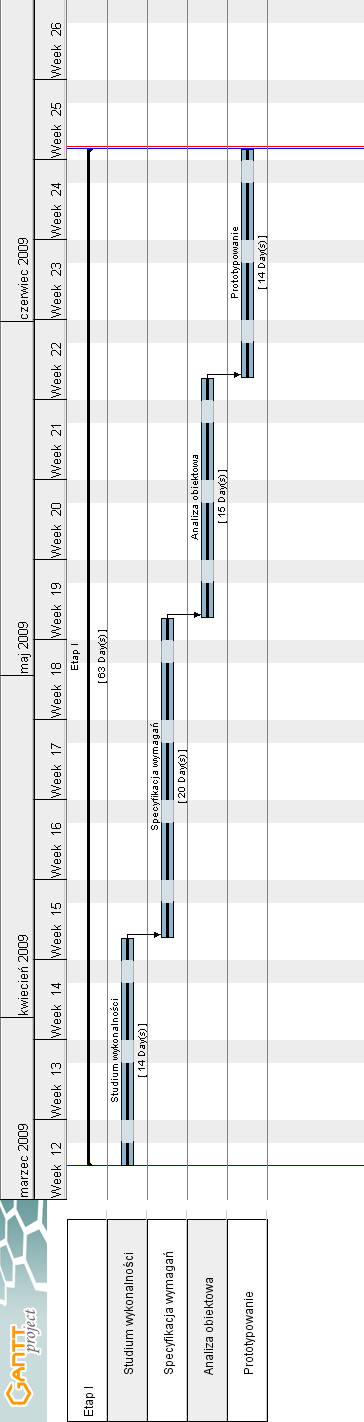
\includegraphics{./img/harmonogramy/sem1.png}}\end{center}
\subsubsection{Harmonogram na II semestr}
\begin{center}
 \scalebox{0.5}{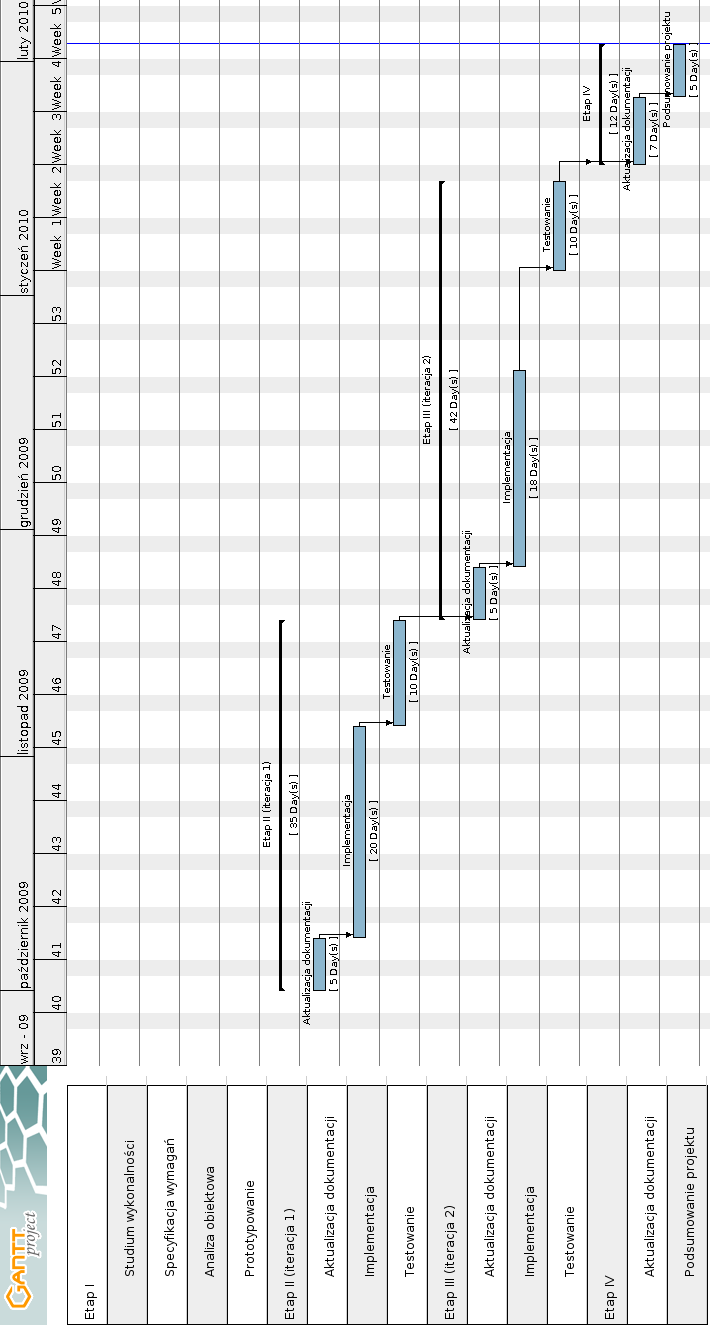
\includegraphics{./img/harmonogramy/sem2.png}}\end{center}




\newpage


%opening
\section{Specyfikacja wymagań systemowych}


\begin{center}
%budowanie tabeli
\begin{tabular}{|p{7cm}|p{7cm}|}
\hline
Symbol projektu: & Opiekun projektu:   \tabularnewline
3@KASK & mgr inż. Tomasz Boiński    \tabularnewline \hline
\multicolumn{2}{|l|}{Nazwa Projektu: } \tabularnewline
\multicolumn{2}{|l|}{Wizualizacja grafów za pomocą biblioteki Prefuse } \tabularnewline
\hline
\multicolumn{2}{l}{ } \tabularnewline %pusta linijka
\hline
Nazwa Dokumentu: & Nr wersji:   \tabularnewline
Specyfikacja wymagań systemowych & 0.9 \tabularnewline \hline
Odpowiedzialny za dokument: & Data pierwszego sporządzenia:   \tabularnewline
Piotr Orłowski & 15 kwietnia 2009 \tabularnewline \hline
Przeznaczenie: & Data ostatniej aktualizacji:   \tabularnewline
DLA KLIENTA & \today \tabularnewline \hline
\end{tabular}
\end{center}


\begin{center}
\begin{tabular}{|c|p{4cm}|c|c|c|}
\multicolumn{5}{c}{\textbf{Historia dokumentu}} \tabularnewline \hline
\textbf{Wersja} & \textbf{Opis modyfikacji} & \textbf{Rozdział/strona} & \textbf{Autor modyfikacji} & \textbf{Data} \tabularnewline \hline
1 & Stworzenie & wszystkie & Grupa projektowa & 15.04.09 \tabularnewline \hline
2 & Wpisanie celów i wymogów ogólnych  & cele & Grupa projektowa & 16.04.09\tabularnewline \hline
3 & Wpisanie funkcjonalnosci wizualizacyjnych & & Grupa projektowa & 28.04.09\tabularnewline \hline
4 & Opis wymagań & & Grupa projektowa & 05.05.09\tabularnewline \hline
5 & Zmiana kolorów Property (SomeValuesFrom i AllValuesFrom) & Projekt wizualizacji & Grupa projektowa & 18.05.09\tabularnewline \hline
6 & WJ001 - klasa Thing w grafie & Wymagania jakościowe & Grupa projektowa & 25.05.09\tabularnewline \hline
7 & Korekta & Całość & Piotr Kunowski & 16.06.09 \tabularnewline \hline
8 & Zmiana wymagać dot. wizualizacji & Projekt wizualizacji & Radosław Kleczkowski & 16.12.09 \tabularnewline \hline
9 & Zmiana wymagać dot. wizualizacji (property) & Projekt wizualizacji & Radosław Kleczkowski & 31.01.10 \tabularnewline \hline
\end{tabular}
\end{center}


\newpage

\subsection{Cele systemu}

%Chociaż cele projektu zostały sformułowane w zleceniu projektowym, to w tym miejscu precyzuje się je z podziałem na cele biznesowe i cele funkcjonalne. Zdarza się tak, że zleceniodawca początkowo wymienia tylko cele funkcjonalne zachowując do swojej wiadomości cele biznesowe. Aby jednak właściwie rozumieć te funkcje w odpowiednim kontekście, zespół projektowy musi poznać motywacje biznesowe klienta.

\subsubsection{Cele biznesowe}




\begin{center}
\begin{tabular}{|m{3cm}|m{9cm}|} \hline

CB001 & Ułatwienie pracy programistom tworzącym aplikacje wizualizujące ontologie  \\ \hline
Opis: & Istnieje zapotrzebowanie na bibliotekę tłumaczącą OWL bezpośrednio na elementy graficzne.  \\ \hline
Źródło: & Wstępna specyfikacja projektu \\ \hline
Priorytet: & bardzo ważne \\ \hline
\multicolumn{2}{c}{} \\

%priorytety  00 01 10 11
%priorytety bardzo wazne, wazne, średnio ważne, mało wazne

 \hline
CB002 & Ułatwienie zakończenia projektu OCS   \\ \hline
Opis: & Moduł wizualizujący ontolgie w OCS wymaga modernizacji i rozbudowy funkcjonalności. Zapewnienie biblioteki wizualizującej ontologie ułatwi i przyspieszy ten proces.  \\ \hline
Źródło:& Klient - mgr inż. Tomasz Boiński   \\ \hline
Priorytet: & bardzo ważne \\ \hline
\multicolumn{2}{c}{} \\
 \hline
CB003 & Zwiększenie aktrakcyjności portalu OCS   \\ \hline
Opis: & Poprawa estetyki modułu wizualizującego ontologię moze przyczynic się do sukcesu portalu po jego wdrożeniu.  \\ \hline
Źródło: & Klient - mgr inż. Tomasz Boiński \\ \hline
Priorytet: & mało ważne \\ \hline
\multicolumn{2}{c}{} \\
\end{tabular}

%\begin{tabular}{|m{3cm}|m{9cm}|} \hline
%CB004 &    \\ \hline
%Opis: &   \\ \hline
%Źródło: &  \\ \hline
%Priorytet: & \\ \hline
%\end{tabular}

\end{center}

\subsubsection{Cele funkcjonalne}

%Cele funkcjonalne wymieniają główne funkcje, które ma spełniać system.

\begin{center}

\begin{tabular}{|m{3cm}|m{9cm}|} \hline

CF001 & Intuicyjne API \\ \hline
Opis: & API powinno być uznane za intuicyjne w opinii członków zespołu i klienta. \\ \hline
Źródło: & Klient - mgr inż. Tomasz Boiński \\ \hline
Priorytet: & średnio ważne  \\ \hline
\multicolumn{2}{c}{} \\

 \hline
CF002 & Dobra dokumentacja \\ \hline
Opis: & Przygotowanie dokumentacji w Javadoc ułatwi pracę użytkownikom biblioteki. \\ \hline
Źródło: & Klient - mgr inż. Tomasz Boiński  \\ \hline
Priorytet: & bardzo ważne \\ \hline

\multicolumn{2}{c}{} \\
 \hline
CF003 & Wizualizacja ontologii \\ \hline
Opis: & Stworzenie biblioteki, która pozwoli na wizualizacje obiektów OWL API przy użyciu odpowiedniej biblioteki graficznej. \\ \hline
Źródło:  & Specyfikacja projektu  \\ \hline
Priorytet: & bardzo ważne \\ \hline

\multicolumn{2}{c}{} \\
 \hline
CF004 & Umożliwienie graficznej edycji i dodawania obiektów OWL API \\ \hline
Opis: &  Dostarczenie tej funkcjonalności ułatwi tworzenie programów z interfejsem pozwalającym na edycję ontologii zapisanych w OWL API. \\ \hline
Źródło: & Klient - mgr inż. Tomasz Boiński \\ \hline
Priorytet: & średnio ważne \\ \hline
\multicolumn{2}{c}{} \\


 \hline

CF005 & Udostępnienie informacji do debuggowania  \\ \hline
Opis: &  Biblioteka powinna wysyłać komunikaty informacyjne, ostrzegawcze oraz informujace o błędach na strumień udostępniony użytkownikowi.  \\ \hline
Źródło: & Standard tworzenia biblioteki 
%\footnote{Code conventions for the javatm programming language. publikacja elektroniczna, kwiecień 1999.
%\url{http://java.sun.com/docs/codeconv/html/CodeConventions.doc8.html}
%}
 \\ \hline
Priorytet: & średnio ważne \\ \hline

\end{tabular}

\end{center}

\subsection{Otoczenie systemu}

%Zespół projektowy musi poznać otoczenie, w jakim ma pracować system. Z rozmów z klientem powinno dać się wyszczególnić użytkowników oraz systemy zewnętrzne. Jeśli się nie da, to otoczenie systemu trzeba będzie zdefiniować w trakcie analizy funkcjonalnej.

\subsubsection{Użytkownicy}

Specyfika projektu nie definiuje użytkowników systemu.

%\begin{tabular}{|m{3cm}|m{9cm}|} \hline

%Tutaj jest ID & A tutaj nazwa \\ \hline
%Opis: &  \\ \hline
%Potrzeby: &  \\ \hline
%Zadania: &  \\ \hline
%Źródło: &  \\ \hline
%Priorytet: &  \\ \hline

%\end{tabular}


\subsubsection{Systemy zewnętrzne}

Specyfika systemu nie wymaga definiowaia systemów zewnętrznych.

%\begin{center}
%\begin{tabular}{|m{3cm}|m{9cm}|} \hline

%Tutaj jest ID & A tutaj nazwa \\ \hline
%Opis: &  \\ \hline
%Interfejsy: &  \\ \hline
%Źródło: &  \\ \hline
%Priorytet: &  \\ \hline

%\end{tabular}
%\end{center}

\subsection{Przewidywane komponenty systemu}

%Wyszczególnienie komponentów systemu powinno pomóc w uzyskaniu kompletności wymagań. Trzeba wówczas sprawdzić, czy każdy komponent ma jakieś wymagania (zwłaszcza funkcjonalne). W przypadku bardziej złożonego systemu może być konieczne wyszczególnienie podsystemów.

\subsubsection{Podsystemy}
Specyfika projektu sprawia, że podsystemy nie będa rozpatrywane.

\subsubsection{Komponenty sprzętowe}
Specyfika projektu sprawia, że komponenty sprzętowe nie będa rozpatrywane.

\subsubsection{Programowe}

\begin{center}
\begin{tabular}{|m{3cm}|m{9cm}|} \hline

KS001 & Prefuse \\ \hline
Opis: &  Biblioteka graficzna do wizualizacji grafów w języku Java\\ \hline
Powiązania: &  \\ \hline
Źródło: & Specyfikacja projektu \\ \hline
Priorytet: & bardzo ważne \\ \hline

\multicolumn{2}{c}{} \\
 \hline

KS002 & OWL API \\ \hline
Opis: &  Biblioteka do przetwarzania ontologii zapisanych w języku OWL. Napisana w języku Java.\\ \hline
Powiązania: &  \\ \hline
Źródło: & Specyfikacja projektu \\ \hline
Priorytet: & bardzo ważne \\ \hline


\end{tabular}
\end{center}

\subsection{Wymagania funkcjonalne}

%Wymagania funkcjonalne stanowią mocno rozbudowaną część specyfikacji. Można je podzielić na grupy dotyczące różnych zadań, różnych użytkowników (systemów zewnętrznych) albo różnych komponentów.

\begin{center}

\begin{tabular}{|m{3cm}|m{9cm}|} \hline

WF001 & Udostępnienie kilku algorytmów wizualizacji \\ \hline
Opis: & Biblioteka powinna udostępniać kilka trybów prezentacji grafów (np. w formie drzewa, w formie gwiazdy i innych).    \\ \hline
Dotyczy: & CF003 \\ \hline
Źródło: & klient - mgr Tomasz Boiński \\ \hline
Powiązania: &WF002 \\ \hline
Priorytet: & średnio ważny\\ \hline

\multicolumn{2}{c}{} \\
 \hline

WF002 & Parametryzacja trybów wizualizacyjnych \\ \hline
Opis: & Domyślne parametry w trybach wizualizacji (takie jak długość krawędzi grafu, automatyczne układanie) powinny zostać dobrane w taki sposób, by obraz był przejrzysty, stabilny i czytelny.    \\ \hline
Dotyczy: & CF003 \\ \hline
Źródło: &  klient - mgr Tomasz Boiński\\ \hline
Powiązania: & WF001 \\ \hline
Priorytet: & średnio ważny \\ \hline

\multicolumn{2}{c}{} \\
 \hline

WF003 & Udostępnienie strumienia błędów \\ \hline
Opis: &   Biblioteka będzie udostępniać strumień danych, w którym znajdą się komunikaty o błędach. Strumień ten będzie mógł zostać wykorzystany przez użytkownika. \\ \hline
Dotyczy: &  CF005  \\ \hline
Źródło: & klient - mgr inż. Tomasz Boiński \\ \hline
Powiązania: & \\ \hline
Priorytet: & ważne \\ \hline

\multicolumn{2}{c}{} \\
 \hline

WF010 & Dodatkowe informacje \\ \hline
Opis: &   Biblioteka będzie dostarczać informacje o wersji ontologii zapisane w pliku OWL oraz dodatkowe informacje o klasach (annotationProperty). \\ \hline
Dotyczy: &  CF003  \\ \hline
Źródło: & klient - mgr inż. Tomasz Boiński \\ \hline
Powiązania: & \\ \hline
Priorytet: & średnio ważne \\ \hline

\end{tabular}

\end{center}

\subsubsection{Wymagania wizualizacji ontologii}

\begin{center}
\begin{tabular}{|m{3cm}|m{9cm}|} \hline

WF004 & Rozróżnialność podstawowych symboli  \\ \hline
Opis: &  Class, Individual, Property powinny mieć rozróżnialne symbole   \\ \hline
Dotyczy: &  CF003 \\ \hline
Źródło: &  klient - mgr inż. Tomasz Boiński\\ \hline
Powiązania: & \\ \hline
Priorytet: & bardzo ważne \\ \hline
%Projekt: & \includegraphics{myimage.png}

\multicolumn{2}{c}{} \\
 \hline

WF005 &   Rozróżnialność szczególnych typów Class\\ \hline
Opis: &   Klasa anonimowa, datatype, Thing i Nothing powinny być łatwo rozpoznawalne.  \\ \hline
Dotyczy: &  CF003 \\ \hline
Źródło: &  klient - mgr inż. Tomasz Boiński\\ \hline
Powiązania: & WF004 \\ \hline
Priorytet: &  ważne \\ \hline

\multicolumn{2}{c}{} \\
 \hline

WF006 &  Rozróżnialność związków między klasami (Class), instancjami (Individual) oraz predykatami (Property)\\ \hline
Opis: & Rózne symobole dla equivalentClass, disjointWith, subClassOf, sameAs, differentFrom, allDifferent, oneOf, unionOf, intersectionOf, complementOf, subProperty, equivalentProperty, hasProperty.   \\ \hline
Dotyczy: &  CF003\\ \hline
Źródło: &  klient - mgr inż. Tomasz Boiński \\ \hline
Powiązania: & WF005, WF004 \\ \hline
Priorytet: & ważne \\ \hline

\multicolumn{2}{c}{} \\
 \hline

WF007 & Rozróżnialność ograniczeń predykatów (Restrictions) \\ \hline
Opis: & Wyróżnić kardynalność (cardinality), domeny (domains) predykatów, inverseOf, właściwości predykatów (transitive, symmetric, functional, inverseFunctional). \\ \hline
Dotyczy: &  CF003\\ \hline
Źródło: &  klient - mgr inż. Tomasz Boiński \\ \hline
Powiązania: & WF004\\ \hline
Priorytet: & ważne \\ \hline

\multicolumn{2}{c}{} \\
 \hline

WF008 &  Podświetlanie wybranych związków i powiazań.\\ \hline
Opis: &   Podświetlać subklasy danej klasy po ich wybraniu myszką po zdefiniowanym zdarzeniu; podobnie subproperty i complex class. \\ \hline
Dotyczy: &  CF003\\ \hline
Źródło: &  klient - mgr inż. Tomasz Boiński \\ \hline
Powiązania: & WF006\\ \hline
Priorytet: & mało ważne \\ \hline

\multicolumn{2}{c}{} \\
 \hline

WF009 & Możliwość definiowania zdarzeń. \\ \hline
Opis: &   Użytkownik będzie mógł pod uchwyty zdarzeń podpinać własne funkcje obsługi. \\ \hline
Dotyczy: & CF003, CF004  \\ \hline
Źródło: & klient - mgr inż. Tomasz Boiński \\ \hline
Powiązania: & \\ \hline
Priorytet: & mało ważne \\ \hline

\end{tabular}

\end{center}

\subsubsection{Projekt wizualizacji}

\begin{longtable}{|c|c|p{7cm}|} \hline
Identyfikator: & Nazwa & Wizualizacja \\ \hline

PW001: & Thing &
 \scalebox{0.30}{
\includegraphics{./img/thing.png}}
 % class.png: 194x86 pixel, 90dpi, 5.48x2.43 cm, bb=0 0 155 69
 \\ \hline

PW002: & Nothing &
 \scalebox{0.30}{
\includegraphics{./img/nothing.png}}
 % class.png: 194x86 pixel, 90dpi, 5.48x2.43 cm, bb=0 0 155 69
 \\ \hline

PW003: & Class &
 \scalebox{0.30}{
\includegraphics{./img/class.png}}
 % class.png: 194x86 pixel, 90dpi, 5.48x2.43 cm, bb=0 0 155 69
 \\ \hline

PW004: & Individual &
 \scalebox{0.30}{
\includegraphics{./img/individual.png}}
 % class.png: 194x86 pixel, 90dpi, 5.48x2.43 cm, bb=0 0 155 69
 \\ \hline

PW005: & Property &
 \scalebox{0.30}{
\includegraphics{./img/property.png}}
 % class.png: 194x86 pixel, 90dpi, 5.48x2.43 cm, bb=0 0 155 69
 \\ \hline

PW006: & Datatype &
 \scalebox{0.30}{
\includegraphics{./img/datatype.png}}
 % class.png: 194x86 pixel, 90dpi, 5.48x2.43 cm, bb=0 0 155 69
 \\ \hline

PW007: & Anonymous Class &
 \scalebox{0.30}{
\includegraphics{./img/anonymousClass.png}}
 % class.png: 194x86 pixel, 90dpi, 5.48x2.43 cm, bb=0 0 155 69
 \\ \hline

PW008: & Subclass &
 \scalebox{0.30}{
\includegraphics{./img/subclass.png}}
 % class.png: 194x86 pixel, 90dpi, 5.48x2.43 cm, bb=0 0 155 69
 \\ \hline

PW009: & instanceOf &
 \scalebox{0.30}{
\includegraphics{./img/instanceOf.png}} \newline
 \scalebox{0.30}{
\includegraphics{./img/instanceOfDatatype.png}}
 % class.png: 194x86 pixel, 90dpi, 5.48x2.43 cm, bb=0 0 155 69
 \\ \hline

PW010: & equivalentClass &
 \scalebox{0.30}{
\includegraphics{./img/equivalentClass.png}}
 % class.png: 194x86 pixel, 90dpi, 5.48x2.43 cm, bb=0 0 155 69
 \\ \hline

PW011: & disjointWith &
 \scalebox{0.30}{
\includegraphics{./img/disjointWith.png}}
 % class.png: 194x86 pixel, 90dpi, 5.48x2.43 cm, bb=0 0 155 69
 \\ \hline

PW012: & differentFrom / allDifferent &
 \scalebox{0.30}{
\includegraphics{./img/allDifferent.png}}
 % class.png: 194x86 pixel, 90dpi, 5.48x2.43 cm, bb=0 0 155 69
 \\ \hline

PW013: & sameAs &
 \scalebox{0.30}{
\includegraphics{./img/sameAs.png}}
 % class.png: 194x86 pixel, 90dpi, 5.48x2.43 cm, bb=0 0 155 69
 \\ \hline

PW014: & oneOf &
 \scalebox{0.30}{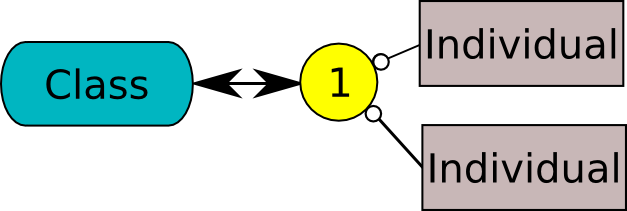
\includegraphics{./img/oneOf.png}}
 % class.png: 194x86 pixel, 90dpi, 5.48x2.43 cm, bb=0 0 155 69
 \\ \hline

PW015: & unionOf &
 \scalebox{0.30}{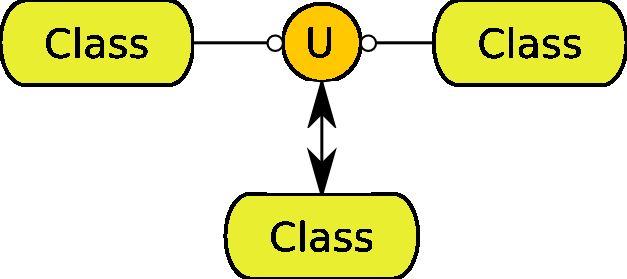
\includegraphics{./img/unionOf.png}}
 % class.png: 194x86 pixel, 90dpi, 5.48x2.43 cm, bb=0 0 155 69
 \\ \hline

PW016: & intersectionOf &
 \scalebox{0.30}{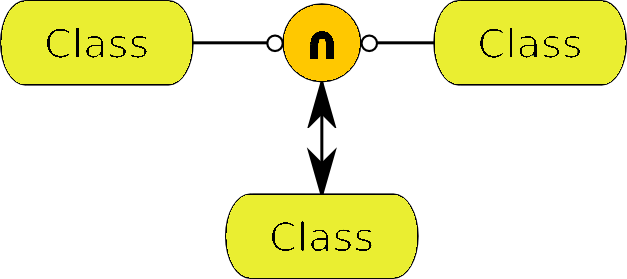
\includegraphics{./img/intersectionOf.png}}
 % class.png: 194x86 pixel, 90dpi, 5.48x2.43 cm, bb=0 0 155 69
 \\ \hline

PW017: & complementOf &
 \scalebox{0.30}{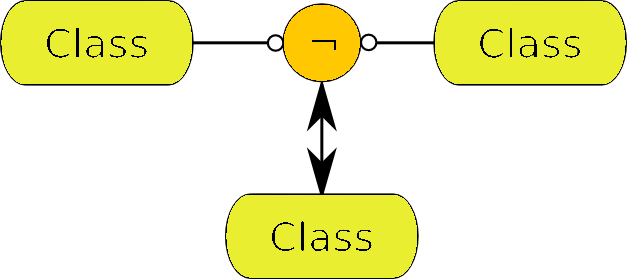
\includegraphics{./img/complementOf.png}}
 % class.png: 194x86 pixel, 90dpi, 5.48x2.43 cm, bb=0 0 155 69
 \\ \hline

PW018: & subProperty &
 \scalebox{0.30}{
\includegraphics{./img/subProperty.png}}
 % class.png: 194x86 pixel, 90dpi, 5.48x2.43 cm, bb=0 0 155 69
 \\ \hline

PW019: & inverseOf (property) &
 \scalebox{0.30}{
\includegraphics{./img/inverseOf.png}} \newline
\scalebox{0.30}{
\includegraphics{./img/inverseOfProperty.png}}
 % class.png: 194x86 pixel, 90dpi, 5.48x2.43 cm, bb=0 0 155 69
 \\ \hline

PW020: & equivalentProperty &
 \scalebox{0.30}{
\includegraphics{./img/equivalentProperty.png}}
 % class.png: 194x86 pixel, 90dpi, 5.48x2.43 cm, bb=0 0 155 69
 \\ \hline

PW021: & functionalProperty &
 \scalebox{0.30}{
\includegraphics{./img/functionalProperty.png}}
 % class.png: 194x86 pixel, 90dpi, 5.48x2.43 cm, bb=0 0 155 69
 \\ \hline

PW022: & inverseFunctionalProperty &
 \scalebox{0.30}{
\includegraphics{./img/inverseFunctionalProperty.png}}
 % class.png: 194x86 pixel, 90dpi, 5.48x2.43 cm, bb=0 0 155 69
 \\ \hline

PW023: & symmetricProperty &
 \scalebox{0.30}{
\includegraphics{./img/symmetricProperty.png}}
 % class.png: 194x86 pixel, 90dpi, 5.48x2.43 cm, bb=0 0 155 69
 \\ \hline

PW024: & transitiveProperty &
 \scalebox{0.30}{
\includegraphics{./img/transitiveProperty.png}}
 % class.png: 194x86 pixel, 90dpi, 5.48x2.43 cm, bb=0 0 155 69
 \\ \hline

PW025: & hasProperty &
 \scalebox{0.25}{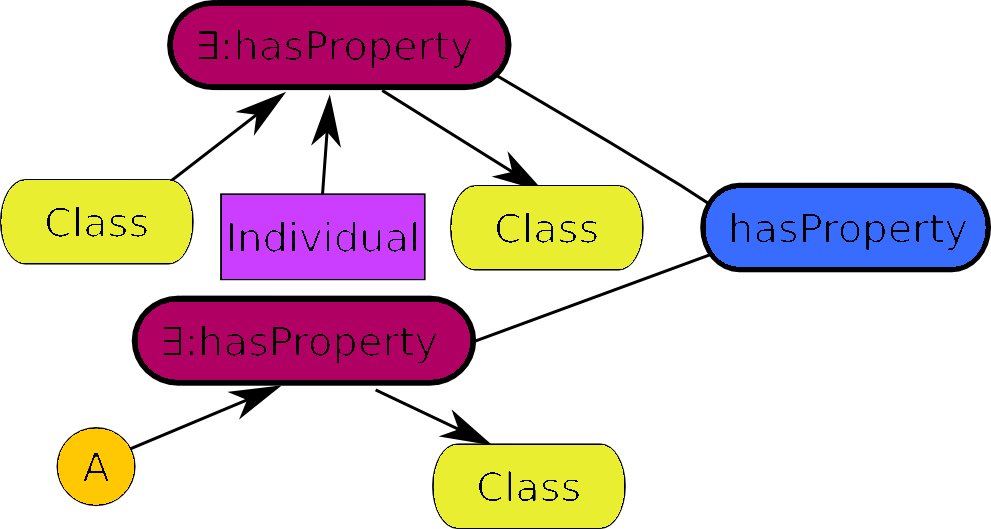
\includegraphics{elementyGraficzne/hasProperty3.png}} 
 %\newline
%\scalebox{0.25}{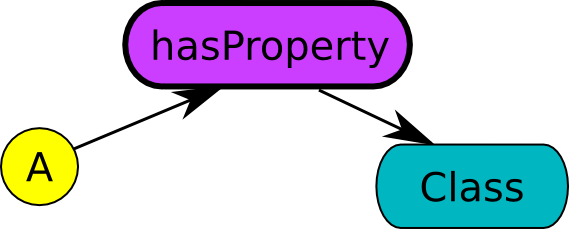
\includegraphics{elementyGraficzne/hasProperty2.png}}
 % class.png: 194x86 pixel, 90dpi, 5.48x2.43 cm, bb=0 0 155 69
 \\ \hline

PW026: & domain &
 \scalebox{0.25}{
\includegraphics{./img/domain.png}}
 % class.png: 194x86 pixel, 90dpi, 5.48x2.43 cm, bb=0 0 155 69
 \\ \hline

PW027: & range &
 \scalebox{0.25}{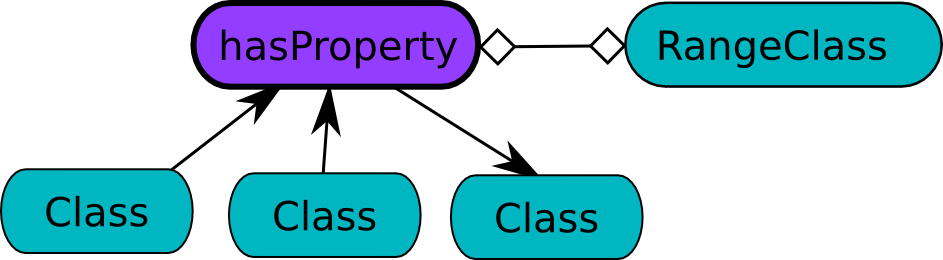
\includegraphics{./img/range.png}}
 % class.png: 194x86 pixel, 90dpi, 5.48x2.43 cm, bb=0 0 155 69
 \\ \hline

PW028: & allValuesFrom &
 \scalebox{0.25}{
\includegraphics{./img/allValuesFrom.png}}
 % class.png: 194x86 pixel, 90dpi, 5.48x2.43 cm, bb=0 0 155 69
 \\ \hline

PW029: & someValuesFrom &
 \scalebox{0.25}{
\includegraphics{./img/someValuesFrom.png}}
 % class.png: 194x86 pixel, 90dpi, 5.48x2.43 cm, bb=0 0 155 69
 \\ \hline

PW030: & minCardinality / maxCardinality &
 \scalebox{0.30}{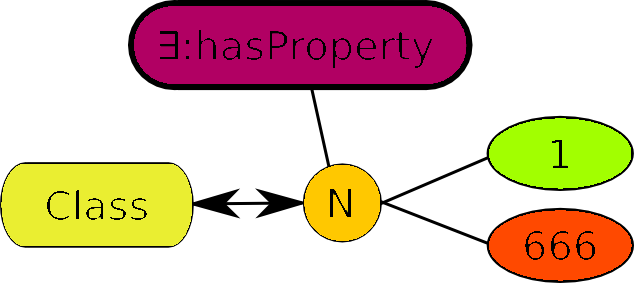
\includegraphics{./img/cardinalityminmax.png}}
 % class.png: 194x86 pixel, 90dpi, 5.48x2.43 cm, bb=0 0 155 69
 \\ \hline

PW031: & cardinality &
 \scalebox{0.30}{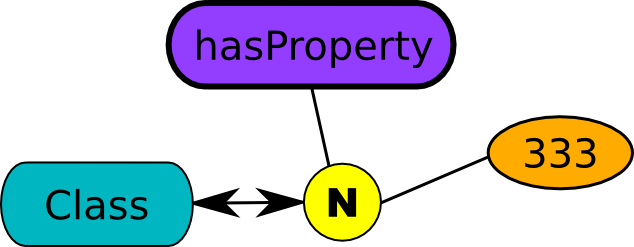
\includegraphics{./img/cardinality.png}}
 % class.png: 194x86 pixel, 90dpi, 5.48x2.43 cm, bb=0 0 155 69
 \\ \hline


\end{longtable}
%\scalebox{0.16}{
\includegraphics{./img/individual.jpg}} \\ \hline
%Projekt: & \includegraphics{myimage.png}




\subsection{Wymagania na dane}

%Wymagania na dane pomagają w określeniu, jakie dane będą przetwarzane w systemie. Nie trzeba precyzować wszystkich danych. Szczegóły znajdą się w projekcie bazy danych.

\begin{center}

\begin{tabular}{|m{3cm}|m{9cm}|} \hline

WD001 & Obsługa obiektów OWL API \\ \hline
Opis: & Biblioteka będzie przystosowana do pobierania, obróbki i zwracania obiektów OWL API. \\ \hline
Powiązania: &  \\ \hline
Źródło: & Klient - mgr inż. Tomasz Boiński  \\ \hline
Priorytet: &  bardzo ważne \\ \hline

\end{tabular}

\end{center}

\subsection{Wymagania jakościowe}

%Określenie wymagań jakościowych ułatwia późniejsze uzyskanie wysokiej jakości systemu. Podział wymagań jakościowych na kategorie jest związany z drzewem jakości (dotyczy wszystkich gałęzi drzewa za wyjątkiem funkcjonalności).

\subsubsection{Wymagania w zakresie wiarygodności}

%Wymagania w zakresie wiarygodności będą rozszerzały wymagania funkcjonalne.


\begin{center}

\begin{tabular}{|m{3cm}|m{9cm}|} \hline

WJ001 & Poprawność wizualizacji \\ \hline
Opis: & Wszystkie wizualizowane elementy powinny pochodzić z ontologii otrzymanej na wejściu programu. Program nie powinien dodawać własnych elementów (np. wywnioskowanych). Wyjątkowo dla klas, które nie mają zdefioniowany nadklas zostanie utworzony związek z klasą Thing. \\ \hline
Powiązania: & WJ002 \\ \hline
Źródło: &  klient - mgr inż. Tomasz Boiński \\ \hline
Priorytet: & bardzo ważne \\ \hline

\multicolumn{2}{c}{} \\
 \hline

WJ002 & Kompletność wizualizacji \\ \hline
Opis: & Jeżeli biblioteka nie wizualizuje danej funkcji OWL API informacja o tym powinna znaleźć się w strumieniu błędów. \\ \hline
Powiązania: & CF005, WJ001, WD001 \\ \hline
Źródło: & klient - mgr inż. Tomasz Boiński \\ \hline
Priorytet: & ważne \\ \hline

\end{tabular}

\end{center}

\subsubsection{Wymagania w zakresie wydajności}

%Wymagania w zakresie wydajności będą miały zastosowanie w czasie projektowania architektury systemu.

Brak wymogów wydajnościowych ze względu na specyfikę projektu.

%\begin{tabular}{|m{3cm}|m{9cm}|} \hline

%Tutaj jest ID & A tutaj nazwa \\ \hline
%Opis: &  \\ \hline
%Powiązania: &  \\ \hline
%Źródło: klient - mgr inż. Tomasz Boiński &  \\ \hline
%Priorytet: &  \\ \hline

%\end{tabular}


\subsubsection{Wymagania w zakresie elastyczności}

%Wymagania w zakresie elastyczności będą miały zastosowanie w czasie wyboru koncepcji systemu.

\begin{center}

\begin{tabular}{|m{3cm}|m{9cm}|} \hline

WJ003 & Obsługiwane wersje Javy \\ \hline
Opis: & Biblioteka powinna wspierać wersje Javy 1.5 i nowsze.\\ \hline
Powiązania: &  \\ \hline
Źródło: & klient - mgr inż. Tomasz Boiński \\ \hline
Priorytet: & bardzo ważne \\ \hline

\multicolumn{2}{c}{} \\
 \hline

WJ004 & Obsługiwane wersje OWL API \\ \hline
Opis: & Powinna istnieć możliwość podpięcia zewnętrznego OWL API (wybranego przez użytkownika/programistę).\\ \hline
Powiązania: &  \\ \hline
Źródło: & klient - mgr inż. Tomasz Boiński \\ \hline
Priorytet: & bardzo ważne \\ \hline

\end{tabular}

\end{center}

\subsubsection{Wymagania w zakresie użyteczności}

%Wymagania w zakresie użyteczności będą brane pod uwagę głównie w czasie projektowania interfejsu użytkownika.

%Ze względu na przyjętą metodykę wytwarzania oprogramowania zagadnienie to zostanie rozpatrzone w przyszłości.
Ze względu specyfikę projektu sytuacje wyjątkowe nie będą rozpatrywane.

%\begin{tabular}{|m{3cm}|m{9cm}|} \hline

%Tutaj jest ID & A tutaj nazwa \\ \hline
%Opis: &  \\ \hline
%Powiązania: &  \\ \hline
%Źródło: &  \\ \hline
%Priorytet: &  \\ \hline

%\end{tabular}


\subsection{Sytuacje wyjątkowe}

%Sytuacje wyjątkowe stanowią dalsze rozszerzenie wymagań funkcjonalnych i wiarygodnościowych.

Ze względu specyfikę projektu sytuacje wyjątkowe nie będą rozpatrywane.

%\begin{tabular}{|m{3cm}|m{9cm}|} \hline

%Tutaj jest ID & A tutaj nazwa \\ \hline
%Opis: &  \\ \hline
%Powiązania: &  \\ \hline
%Źródło: &  \\ \hline
%Priorytet: &  \\ \hline

%\end{tabular}


\subsection{Dodatkowe wymagania}

%W tym miejscu podaje się te wymagania, które nie mieszczą się w zakresie poprzednich kategorii wymagań.

\subsubsection{Wymagania sprzętowe}

%Wymagania sprzętowe można by umieścić w ramach specyfikacji komponentów sprzętowych, ale jeśli jest wiele komponentów sprzętowych różnych z punktu widzenia funkcjonalnego, ale o wspólnych wymaganiach sprzętowych, to można te wymagania umieścić właśnie tutaj.

Ze względu na specyfikę projektu wymagania sprzętowe nie będą rozpatrywane.

%\begin{tabular}{|m{3cm}|m{9cm}|} \hline

%Tutaj jest ID & A tutaj nazwa \\ \hline
%Opis: &  \\ \hline
%Dotyczy: &  \\ \hline
%Źródło: &  \\ \hline
%Priorytet: &  \\ \hline

%\end{tabular}


\subsubsection{Wymagania programowe}

%Trzeba odróżniać rzeczywiste wymagania programowe klienta od jego sugestii (np. przez podanie opcjonalnego priorytetu).

\begin{center}

\begin{tabular}{|m{3cm}|m{9cm}|} \hline

WD003 & JVM \\ \hline
Opis: & Do skorzystania z biblioteki niezbędna jest JVM.\\ \hline
Dotyczy: & CF001, CF002 \\ \hline
Źródło: & klient - mgr inż. Tomasz Boiński \\ \hline
Priorytet: & ważne \\ \hline

\end{tabular}

\end{center}

\subsubsection{Inne wymagania}

\begin{center}

\begin{tabular}{|m{3cm}|m{9cm}|} \hline

WI001 & Dokumentacja w javadoc \\ \hline
Opis: & Wszystkie ważne klasy i funkcje powinny mieć odpowiednią dokumentację w formacie javadoc.\\ \hline
Dotyczy: & CF001, CF002 \\ \hline
Źródło: & klient - mgr inż. Tomasz Boiński \\ \hline
Priorytet: & ważne \\ \hline

\multicolumn{2}{c}{} \\
 \hline

WI002 & Dokumentacja w języku angielskim \\ \hline
Opis: & Dokumentacja wszystkich funkcji i klas powinna posiadać angielską wersję językową.\\ \hline
Dotyczy: & CF001, CF002 \\ \hline
Źródło: & klient - mgr inż. Tomasz Boiński \\ \hline
Priorytet: & mało ważne \\ \hline

\multicolumn{2}{c}{} \\
 \hline

WI003 & Dokumentacja w języku polskim \\ \hline
Opis: & Dokumentacja wszystkich funkcji i klas powinna posiadać polską wersję językową. \\ \hline
Dotyczy: & CF001, CF002 \\ \hline
Źródło: & klient - mgr inż. Tomasz Boiński \\ \hline
Priorytet: & ważne \\ \hline

\multicolumn{2}{c}{} \\
 \hline
WI004 & Nazwy zmiennych i funkcji w języku angielskim \\ \hline
Opis: & Nazwy zmiennych i funkcji powinny zostać dobrane w języku angielskim i zgodnie ze standardami programowania w javie %\footnote{Greg    Travis.          Build    your   own     java  library.          publikacja elektroniczna.
%\url{http://www.digilife.be/quickreferences/PT/Build your own Java library.pdf}
%}.
\\ \hline
Dotyczy: & CF001, CF002 \\ \hline
Źródło: & klient - mgr inż. Tomasz Boiński \\ \hline
Priorytet: & ważne \\ \hline

\end{tabular}

\end{center}

\subsection{Kryteria akceptacyjne}

%Tu podać kryteria, jakim zostanie poddany gotowy system przed ostatecznym jego przyjęciem.

\begin{center}

\begin{tabular}{|m{3cm}|m{9cm}|} \hline

KA001 & Spełnione są podstawowe wymagania wymienione w dokumencie SWS \\ \hline
Opis: & Spełnione są wszystkie wymagania ważne i bardzo ważne zdefiniowane w SWS. \\ \hline
Dotyczy: & wszystkie wymagania ważne i bardzo ważne \\ \hline
Źródło: & klient - mgr inż. Tomasz Boiński \\ \hline
Priorytet: & ważne  \\ \hline %skonsultować z klientem

\multicolumn{2}{c}{} \\
 \hline

KA002 & Biblioteka współpracuje z OWL API dostarczonym przez KASK \\ \hline
Opis: & Biblioteka współpracuje z OWL API dostarczonym przez KASK zbudowanym na podstawie OWL API ver 2.1.1\\ \hline
Dotyczy: & WJ004 \\ \hline
Źródło: & klient - mgr inż. Tomasz Boiński \\ \hline
Priorytet: & ważne  \\ \hline %skonsultować z klientem

\end{tabular}

\end{center}



\newpage

\section{Analiza obiektowa}





\begin{center}
%budowanie tabeli
\begin{longtable}{|p{7cm}|p{7cm}|}
\hline
Symbol projektu: & Opiekun projektu:   \tabularnewline 
3@KASK & mgr inż. Tomasz Boiński    \tabularnewline \hline
\multicolumn{2}{|l|}{Nazwa Projektu: } \tabularnewline
\multicolumn{2}{|l|}{Wizualizacja grafów za pomocą biblioteki Prefuse } \tabularnewline 
\hline
\multicolumn{2}{l}{ } \tabularnewline %pusta linijka
\hline 
Nazwa Dokumentu: & Nr wersji:   \tabularnewline 
Analiza obiektowa & 2.0 \tabularnewline \hline
Odpowiedzialny za dokument: & Data pierwszego sporządzenia:   \tabularnewline 
Piotr Kunowski & 23 maja 2009 \tabularnewline \hline
Przeznaczenie: & Data ostatniej aktualizacji:   \tabularnewline 
DLA KLIENTA & \today \tabularnewline \hline
\end{longtable}
\end{center}


\begin{center}
\begin{longtable}{|c|p{4cm}|c|c|c|}
\multicolumn{5}{c}{\textbf{Historia dokumentu}} \tabularnewline \hline
\textbf{Wersja} & \textbf{Opis modyfikacji} & \textbf{Rozdział/strona} & \textbf{Autor modyfikacji} & \textbf{Data} \tabularnewline \hline 
1 & Stworzenie & wszystkie & Grupa projektowa & 23.05.09 \tabularnewline \hline
1.1 & Dodano pakiet Utils & 1, 3 & Anna Jaworska & 2.06.09 \tabularnewline \hline
2 & Dodano zaktualizowane diagramy oraz opisy klas & wszystkie & Grupa projektowa & 16.06.09 \tabularnewline \hline

\end{longtable}
\end{center}


\newpage

\subsection{Pakiety}

\subsubsection{Diagram}
 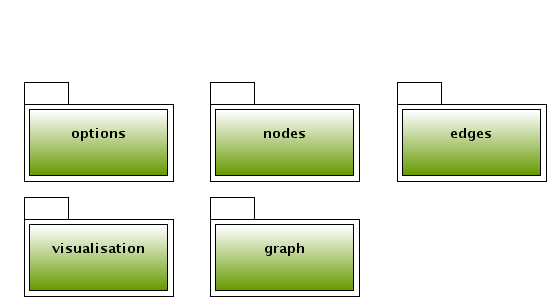
\includegraphics[width=\linewidth]{./modelowanie/OV_UML/PackageDiagram.png}

\newpage
\subsubsection{Opis pakietów}


\begin{center}
\begin{longtable}{|m{3cm}|m{9cm}|} \hline

P001 & options\\ \hline
Opis: & Pakiet zawierający klasy z polami opisującymi różne (modyfikowalne) ustawienia wizualizacji takie jak: kolory, grubość linii itp.     \\ \hline
Interfejsy: &     \\ \hline
Realizowane wymagania: & WF002, WF001, WI004 \\ \hline
Priorytet: & średnio ważne \\ \hline

\multicolumn{2}{c}{} \\
 \hline

P002 & nodes\\ \hline
Opis: & Pakiet z klasami odpowiedzialnymi za wizualizację i przechowywanie danych o wierzchołkach.    \\ \hline
Interfejsy: &     \\ \hline
Realizowane wymagania: & WF004, WF005, WF006, WF007, WI004 \\ \hline
Priorytet: & bardzo ważne \\ \hline

\multicolumn{2}{c}{} \\
 \hline

P003 & edges\\ \hline
Opis: & Pakiet z klasami odpowiedzialnymi za wizualizację i przechowywanie danych o krawędziach.    \\ \hline
Interfejsy: &     \\ \hline
Realizowane wymagania: & WF006, WF007, WI004 \\ \hline
Priorytet: & bardzo ważne \\ \hline

\multicolumn{2}{c}{} \\
 \hline

P004 & visualization\\ \hline
Opis: & Zawiera dodatkowe klasy przydatne w wizualizacji.\\ \hline
Interfejsy: &     \\ \hline
Realizowane wymagania: & WF001, WF008, WI004 \\ \hline
Priorytet: & średnio ważne \\ \hline

\multicolumn{2}{c}{} \\
 \hline

P005 & graph\\ \hline
Opis: & Pakiet zawiera klasy, które zawierają podstawowe operacje na danych OwlApi oraz graph. \\ \hline
Interfejsy: &     \\ \hline
Realizowane wymagania: & WD001 \\ \hline
Priorytet: & bardzo ważne \\ \hline

%\multicolumn{2}{c}{} \\
% \hline
\multicolumn{2}{c}{} \\
 \hline

P006 & utils\\ \hline
Opis: & Pakiet zawiera klasy pomocnicze \\ \hline
Interfejsy: &     \\ \hline
Realizowane wymagania: & CF005 \\ \hline
Priorytet: & bardzo ważne \\ \hline

\end{longtable}

\end{center}

\subsection{Pakiet options}

\subsubsection{Diagram}

 \scalebox{0.50}{ 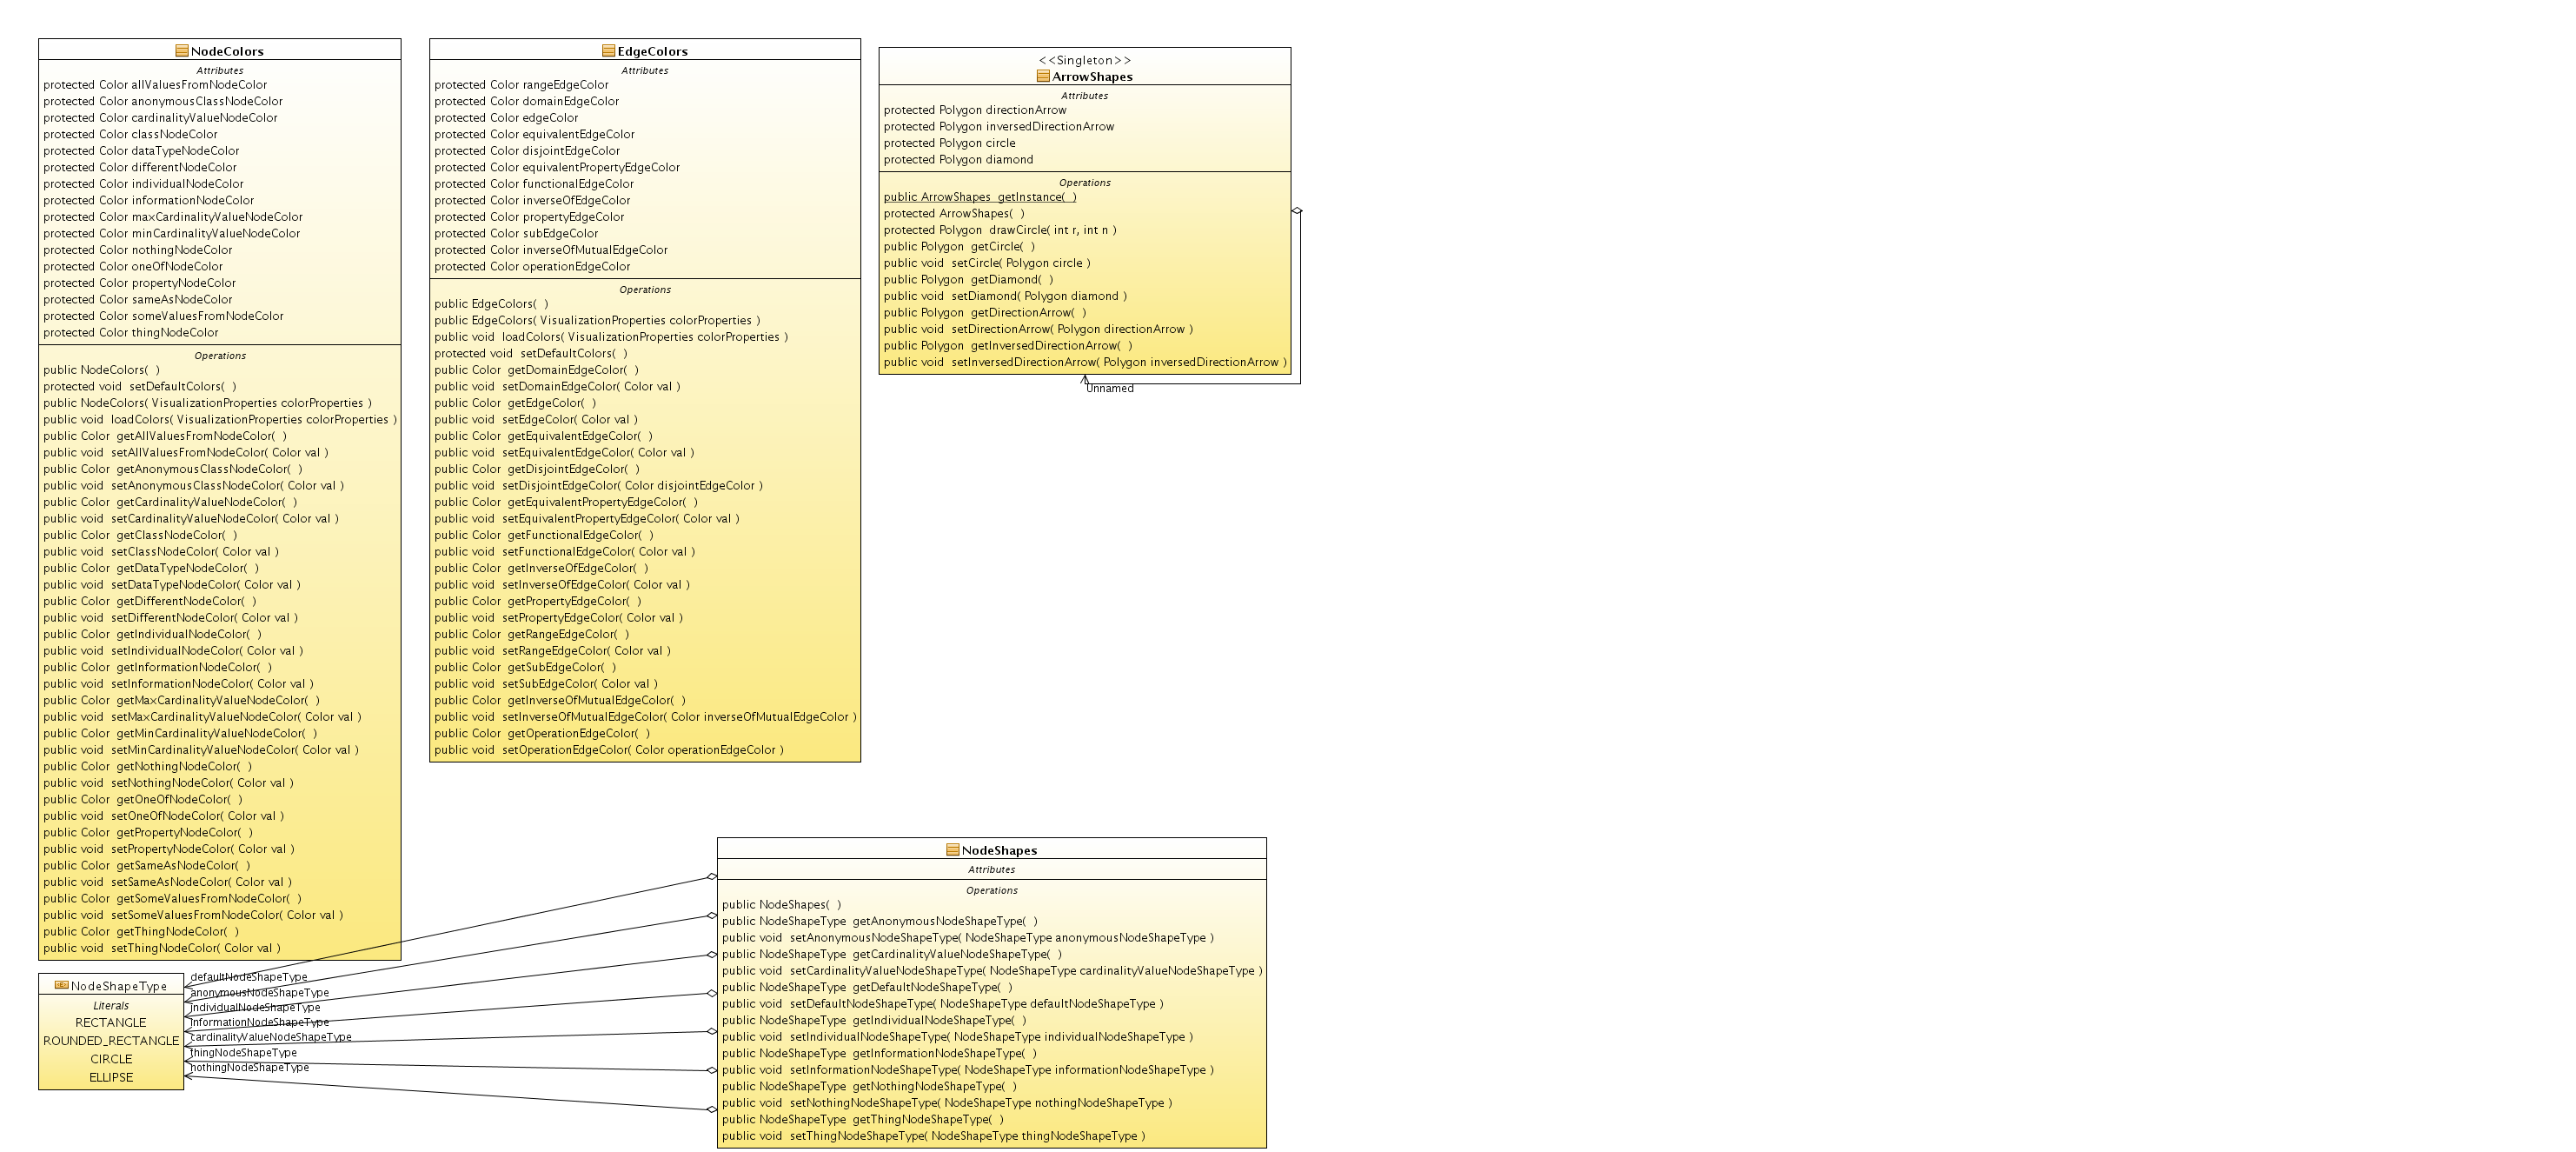
\includegraphics{./modelowanie/OV_UML/OptionsClassDiagram.png}

}

\subsubsection{Opis klasy}

\begin{center}
 


\begin{longtable}{|m{3cm}|m{9cm}|} \hline

CO001 & EdgeColors \\ \hline
Opis: & Zawiera definicje kolorów dla poszczególnych rodzajów krawędzi.   \\ \hline
Klasy nadrzędne: &     \\ \hline
Atrybuty: & \begin{itemize}
 \item domainEdgeColor
 \item edgeColor
 \item equivalentEdgeColor
 \item equivalentPropertyEdgeColor
 \item functionalEdgeColor
 \item inverseOfEdgeColor
 \item propertyEdgeColor
 \item rangeEdgeColor
 \item subEdgeColor

\end{itemize}
 \\ \hline
Metody: & %\begin{itemize}
% \item 
%\end{itemize}
  \\ \hline
Realizowane wymagania: & WF002 \\ \hline
Priorytet: & średnio ważny \\ \hline

\multicolumn{2}{c}{} \\
 \hline

CO002 & NodeColors \\ \hline
Opis: & Zawiera definicje kolorów dla poszczególnych rodzajów krawędzi.   \\ \hline
Klasy nadrzędne: &     \\ \hline
Atrybuty: & \begin{itemize}
 \item allValuesFromNodeColor
 \item cardinalityNodeColor
 \item cardinalityValueNodeColor
 \item classNodeColor
 \item complementOfNodeColor
 \item dataTypeNodeColor
 \item differentNodeColor
 \item functionalPropertyNodeColor
 \item individualNodeColor
 \item informationNodeColor
 \item intersectionOfNodeColor
 \item inverseFunctionalNodeColor
 \item maxCardinalityValueNodeColor
 \item minCardinalityValueNodeColor
 \item nothingNodeColor
 \item oneOfNodeColor
 \item propertyNodeColor
 \item sameAsNodeColor
 \item someValuesFromNodeColor
 \item symmetricPropertNodeColor
 \item thingNodeColor
 \item transitivePropertyNodeColor
 \item unionOfNodeColor 
\end{itemize}
 \\ \hline
Metody: & %\begin{itemize}
 %\item 
%\end{itemize}
  \\ \hline
Realizowane wymagania: & WF002 \\ \hline
Priorytet: & średnio ważny \\ \hline

%\multicolumn{2}{c}{} \\
% \hline

\end{longtable}


\end{center}

\subsection{Pakiet nodes}

\subsubsection{Diagram}

\begin{center}
 \scalebox{0.36}{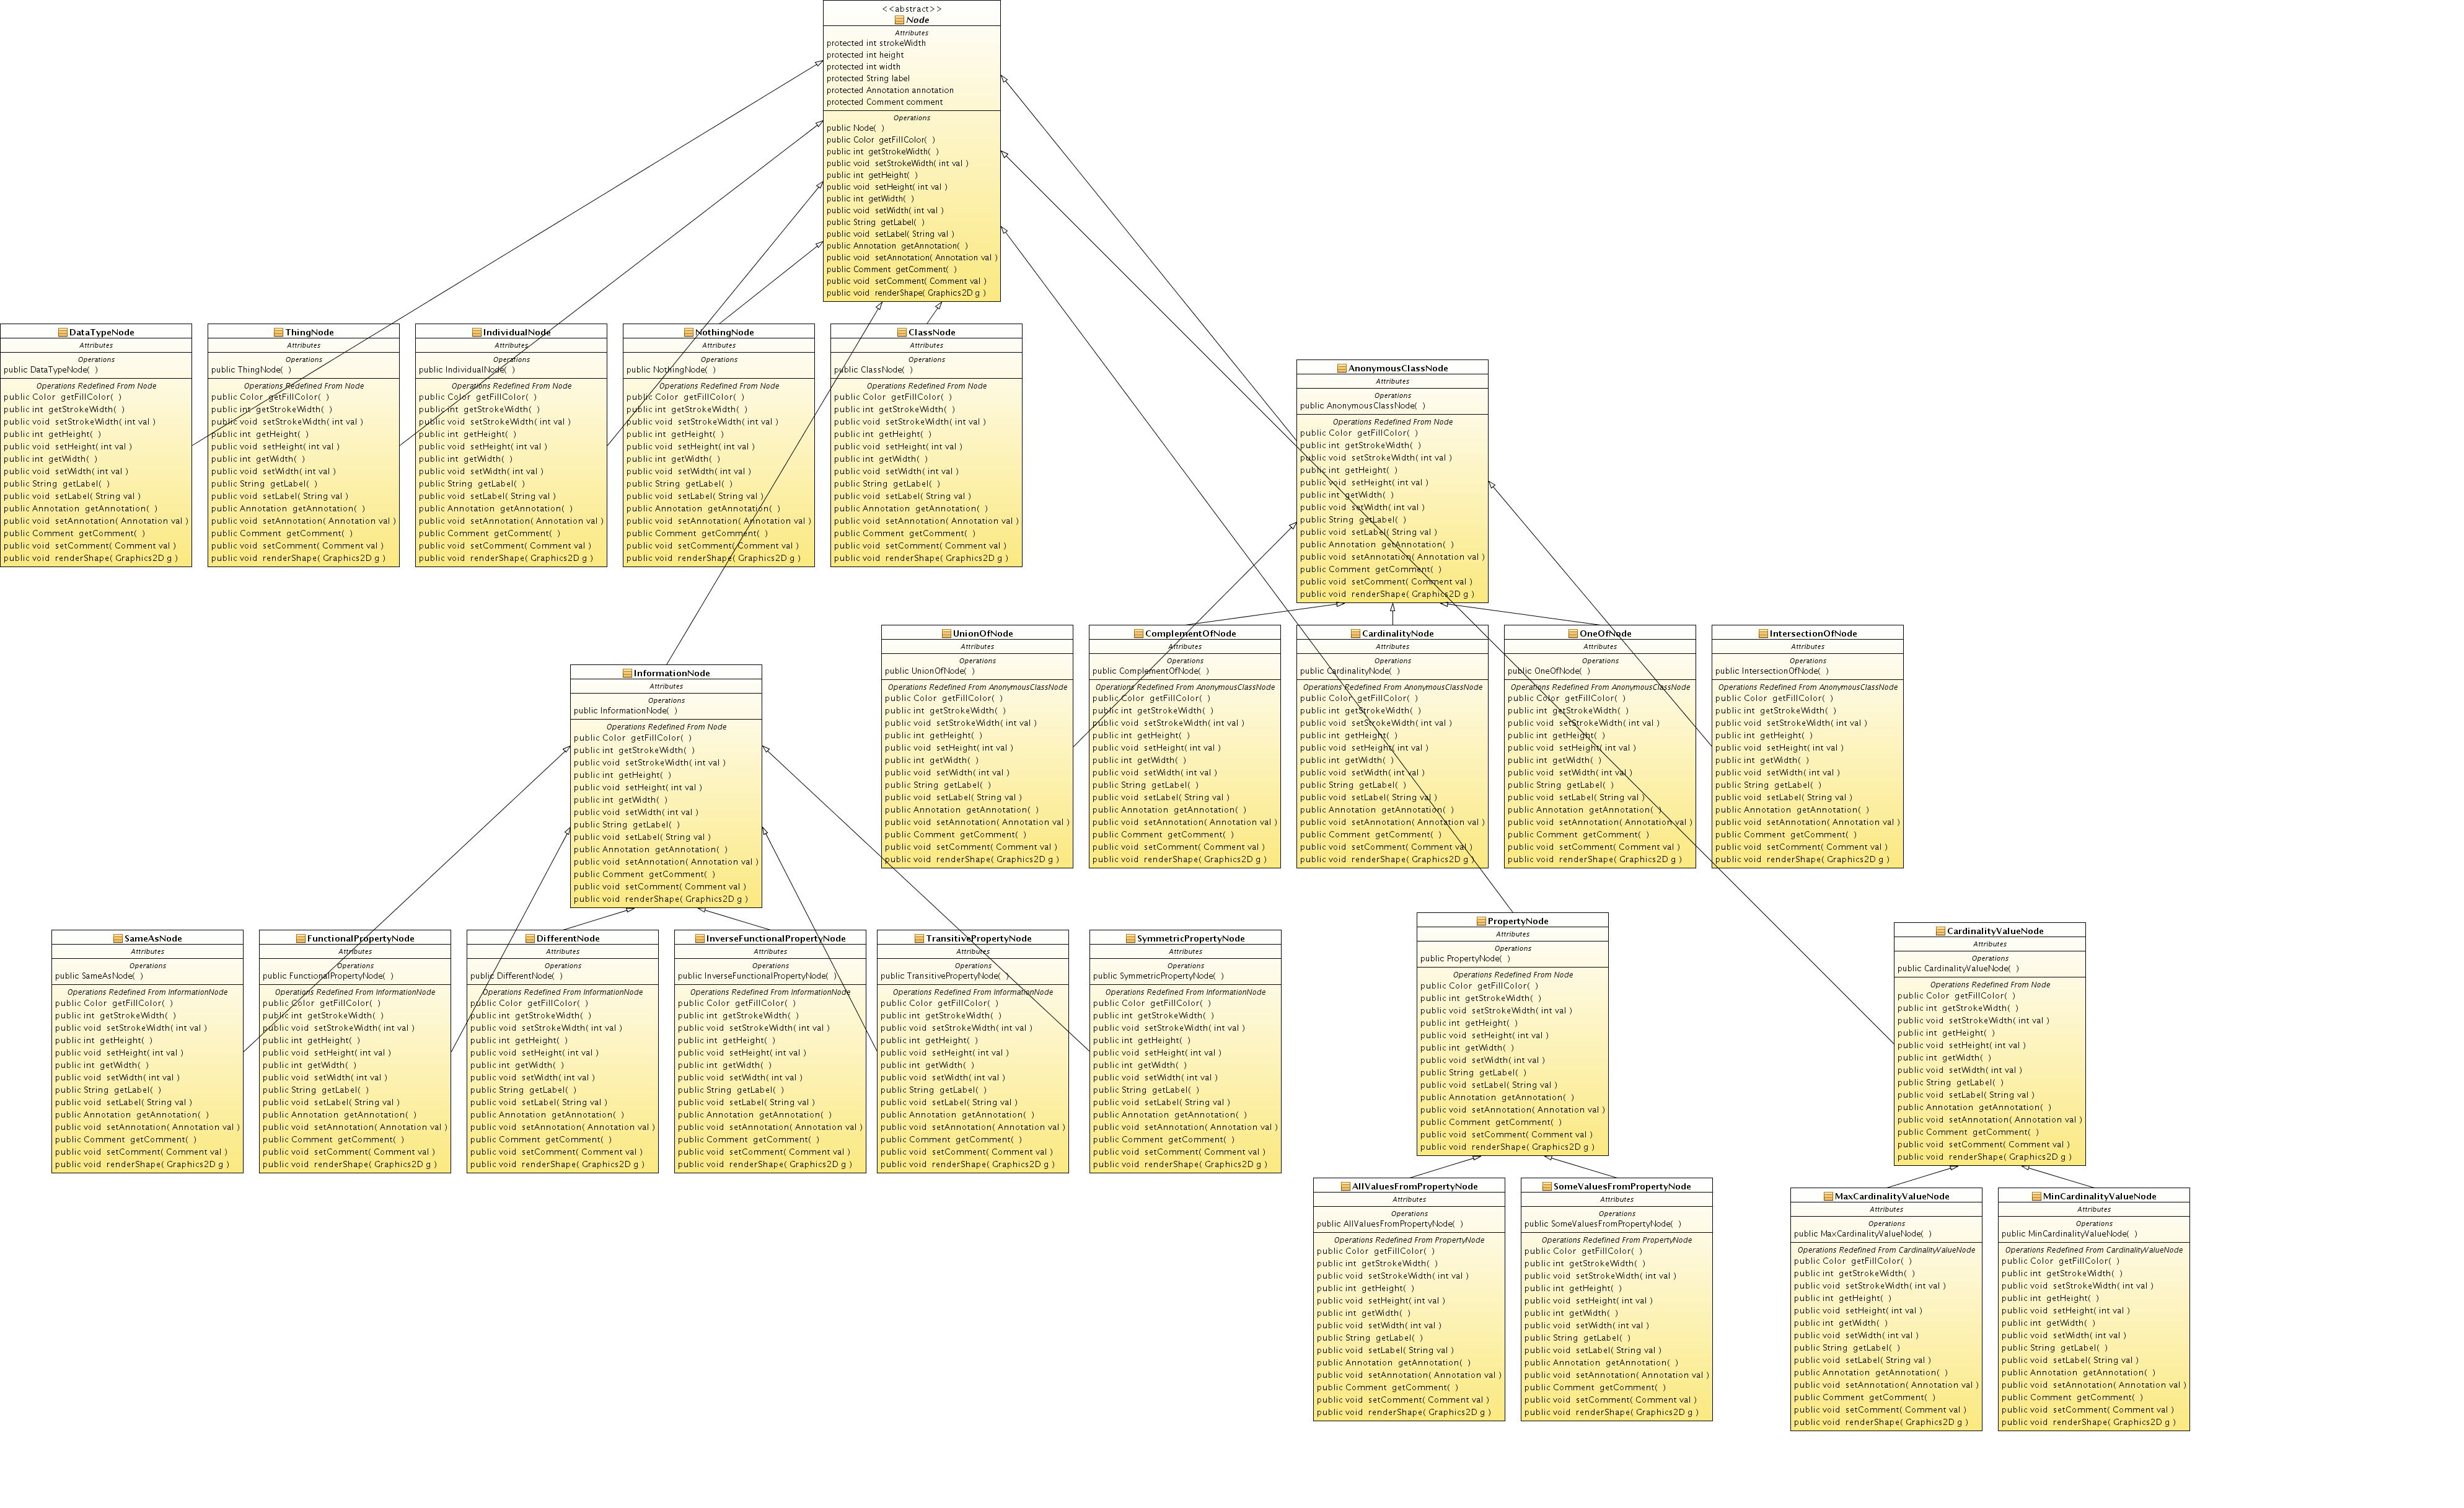
\includegraphics{./modelowanie/OV_UML/NodesClassDiagram.png}}\end{center}

\subsubsection{Opis klasy}

\begin{center}
 


\begin{longtable}{|m{3cm}|m{9cm}|} \hline

CN001 & Node \\ \hline
Opis: & Klasa nadrzędna względem wszystkich klas obsługi wierzchołków. Zawiera definicje podstawowych atrybutów i metod.    \\ \hline
Klasy nadrzędne: &     \\ \hline
Atrybuty: & \begin{itemize}
 \item strokeWidth
 \item height
 \item width
 \item annotation
 \item comment
\item Color fillColor
\item String label
\end{itemize}
 \\ \hline
Metody: &% \begin{itemize}
 %\item renderShape - metoda wizualizująca dany typ wierzchołka
%\end{itemize}
  \\ \hline
Realizowane wymagania: & WF004, WF005, WF006, WF007, WI004 \\ \hline
Priorytet: & bardzo ważne  \\ \hline

\multicolumn{2}{c}{} \\
 \hline

CN002 & AllValuesFromPropertyNode \\ \hline
Opis: & Klasa reprezentuje wierzchołek, będący OWL Property typu AllValuesFrom.    \\ \hline
Klasy nadrzędne: & Node     \\ \hline
Atrybuty: & 
%\begin{itemize}
 %\item 
%\end{itemize}
 \\ \hline
Metody: & %\begin{itemize}
 %\item 
%\end{itemize}
  \\ \hline
Realizowane wymagania: & WF004, WF006, WF007, WI004 \\ \hline
Priorytet: & ważne \\ \hline

\multicolumn{2}{c}{} \\
 \hline

CN003 & AnonymousClassNode \\ \hline
Opis: & Klasa reprezentuje wierzchołek klas anonimowych OWL.    \\ \hline
Klasy nadrzędne: & Node     \\ \hline
Atrybuty: & %\begin{itemize}
 %\item 
%\end{itemize}
 \\ \hline
Metody: & %\begin{itemize}
 %\item 
%\end{itemize}
  \\ \hline
Realizowane wymagania: & WF005, WI004 \\ \hline
Priorytet: & ważne \\ \hline

\multicolumn{2}{c}{} \\
 \hline

CN004 & CardinalityNode \\ \hline
Opis: & Klasa reprezentuje wierzchołek klas anonimowych OWL będących wynikiem ograniczenia kardynalności.    \\ \hline
Klasy nadrzędne: & AnonymousNode     \\ \hline
Atrybuty: & %\begin{itemize}
 %\item 
%\end{itemize}
 \\ \hline
Metody: & %\begin{itemize}
 %\item 
%\end{itemize}
  \\ \hline
Realizowane wymagania: & WF007, WI004 \\ \hline
Priorytet: & ważne  \\ \hline

\multicolumn{2}{c}{} \\
 \hline

CN005 & CardinalityValueNode \\ \hline
Opis: & Klasa reprezentuje wierzchołek z dokładnym ograniczeniem kardynalności (OWL Cardinality). \\ \hline
Klasy nadrzędne: & Node     \\ \hline
Atrybuty: & %\begin{itemize}
 %\item 
%\end{itemize}
 \\ \hline
Metody: & %\begin{itemize}
 %\item 
%\end{itemize}
  \\ \hline
Realizowane wymagania: & WF007, WI004 \\ \hline
Priorytet: & ważne  \\ \hline

\multicolumn{2}{c}{} \\
 \hline

CN006 & ClassNode \\ \hline
Opis: & Klasa reprezentuje wierzchołek OWL Class.    \\ \hline
Klasy nadrzędne: & Node     \\ \hline
Atrybuty: & %\begin{itemize}
 %\item 
%\end{itemize}
 \\ \hline
Metody: & %\begin{itemize}
 %\item 
%\end{itemize}
  \\ \hline
Realizowane wymagania: & WF004, WF005, WI004 \\ \hline
Priorytet: & ważne  \\ \hline

\multicolumn{2}{c}{} \\
 \hline

CN007 & ComplementOfNode \\ \hline
Opis: & Klasa reprezentuje wierzchołek klas anonimowych OWL będących wynikiem dopełnienia (OWL ComplementOf).    \\ \hline
Klasy nadrzędne: & Node     \\ \hline
Atrybuty: & %\begin{itemize}
 %\item 
%\end{itemize}
 \\ \hline
Metody: & %\begin{itemize}
 %\item 
%\end{itemize}
  \\ \hline
Realizowane wymagania: & WF006, WF007, WI004 \\ \hline
Priorytet: & ważne  \\ \hline

\multicolumn{2}{c}{} \\
 \hline

CN008 & DataTypeNode \\ \hline
Opis: & Klasa reprezentuje wierzchołek OWL DataType.    \\ \hline
Klasy nadrzędne: & Node     \\ \hline
Atrybuty: & %\begin{itemize}
 %\item 
%\end{itemize}
 \\ \hline
Metody: & %\begin{itemize}
 %\item 
%\end{itemize}
  \\ \hline
Realizowane wymagania: & WF004, WI04 \\ \hline
Priorytet: & ważne  \\ \hline

\multicolumn{2}{c}{} \\
 \hline

CN009 & DifferentNode \\ \hline
Opis: & Klasa reprezentuje wierzchołek oznaczający relację DifferentFrom lub AllDifferent pomiędzy wystąpieniami klas (OWL Individual).    \\ \hline
Klasy nadrzędne: & Node     \\ \hline
Atrybuty: & %\begin{itemize}
 %\item 
%\end{itemize}
 \\ \hline
Metody: & %\begin{itemize}
 %\item 
%\end{itemize}
  \\ \hline
Realizowane wymagania: & WF006, WF007, WI004 \\ \hline
Priorytet: & ważne  \\ \hline

\multicolumn{2}{c}{} \\
 \hline

CN010 & FunctionalPropertyNode \\ \hline
Opis: & Klasa reprezentuje wierzchołek oznaczający, że dane OWL Property to FunctionalProperty.  \\ \hline
Klasy nadrzędne: & InformationNode     \\ \hline
Atrybuty: & %\begin{itemize}
 %\item 
%\end{itemize}
 \\ \hline
Metody: & %\begin{itemize}
 %\item 
%\end{itemize}
  \\ \hline
Realizowane wymagania: & WF006, WF007, WI004 \\ \hline
Priorytet: & ważne  \\ \hline

\multicolumn{2}{c}{} \\
 \hline

CN011 & IndividualNode \\ \hline
Opis: & Klasa reprezentuje wierzchołek instancji OWL Individual.  \\ \hline
Klasy nadrzędne: & Node     \\ \hline
Atrybuty: & %\begin{itemize}
 %\item 
%\end{itemize}
 \\ \hline
Metody: & %\begin{itemize}
 %\item 
%\end{itemize}
  \\ \hline
Realizowane wymagania: & WF004, WI004 \\ \hline
Priorytet: & ważne  \\ \hline

\multicolumn{2}{c}{} \\
 \hline

CN012 & InformationNode \\ \hline
Opis: & Klasa ta jest klasą nadrzędną, dla klas wierzchołków reprezentujących informacje o różnych właściwościach OWL Property.    \\ \hline
Klasy nadrzędne: & Node     \\ \hline
Atrybuty: & %\begin{itemize}
 %\item 
%\end{itemize}
 \\ \hline
Metody: & %\begin{itemize}
 %\item 
%\end{itemize}
  \\ \hline
Realizowane wymagania: & WF010, WI004 \\ \hline
Priorytet: & ważne  \\ \hline

\multicolumn{2}{c}{} \\
 \hline

CN013 & IntersectionOfNode \\ \hline
Opis: & Klasa reprezentuje wierzchołek klas anonimowych OWL będących wynikiem przecięcia (OWL IntersectionOf).    \\ \hline
Klasy nadrzędne: & AnonymousNode     \\ \hline
Atrybuty: & %\begin{itemize}
 %\item 
%\end{itemize}
 \\ \hline
Metody: & %\begin{itemize}
 %\item 
%\end{itemize}
  \\ \hline
Realizowane wymagania: & WF005, WI004 \\ \hline
Priorytet: & ważne  \\ \hline

\multicolumn{2}{c}{} \\
 \hline

CN014 & inverseFunciotnalPropertyNode \\ \hline
Opis: & Klasa reprezentuje wierzchołek oznaczający, że dane OWL Property to InverseFunctionalProperty.    \\ \hline
Klasy nadrzędne: & InformationNode     \\ \hline
Atrybuty: & %\begin{itemize}
 %\item 
%\end{itemize}
 \\ \hline
Metody: & %\begin{itemize}
 %\item 
%\end{itemize}
  \\ \hline
Realizowane wymagania: & WF007, WI004 \\ \hline
Priorytet: & ważne  \\ \hline

\multicolumn{2}{c}{} \\
 \hline

CN015 & MaxCardinalityValueNode \\ \hline
Opis: & Klasa reprezentuje wierzchołek ograniczenia kardynalności OWL MaxCardinality.    \\ \hline
Klasy nadrzędne: & CardinalityValueNode     \\ \hline
Atrybuty: & %\begin{itemize}
 %\item 
%\end{itemize}
 \\ \hline
Metody: & %\begin{itemize}
 %\item 
%\end{itemize}
  \\ \hline
Realizowane wymagania: & WF007, WI004 \\ \hline
Priorytet: & ważne  \\ \hline

\multicolumn{2}{c}{} \\
 \hline

CN016 & MinCardinalityValueNode \\ \hline
Opis: & Klasa reprezentuje wierzchołek ograniczenia kardynalności OWL MinCardinality.    \\ \hline
Klasy nadrzędne: & CardinalityValueNode     \\ \hline
Atrybuty: & %\begin{itemize}
 %\item 
%\end{itemize}
 \\ \hline
Metody: & %\begin{itemize}
 %\item 
%\end{itemize}
  \\ \hline
Realizowane wymagania: & WF007, WI004 \\ \hline
Priorytet: & ważne  \\ \hline

\multicolumn{2}{c}{} \\
 \hline

CN017 & NothingNode \\ \hline
Opis: & Klasa reprezentuje wierzchołek OWL Nothing.    \\ \hline
Klasy nadrzędne: & Node     \\ \hline
Atrybuty: & %\begin{itemize}
 %\item 
%\end{itemize}
 \\ \hline
Metody: & %\begin{itemize}
 %\item 
%\end{itemize}
  \\ \hline
Realizowane wymagania: & WF004, WF005, WI004 \\ \hline
Priorytet: & ważne  \\ \hline

\multicolumn{2}{c}{} \\
 \hline

CN018 & OneOfNode \\ \hline
Opis: & Klasa reprezentuje wierzchołek klas anonimowych OWL reprezentujących 1 z klas określonego zbioru (wynik OWL OneOf).    \\ \hline
Klasy nadrzędne: & AnonymousClassNode     \\ \hline
Atrybuty: & %\begin{itemize}
 %\item 
%\end{itemize}
 \\ \hline
Metody: & %\begin{itemize}
 %\item 
%\end{itemize}
  \\ \hline
Realizowane wymagania: & WF005, WF006, WI004 \\ \hline
Priorytet: & ważne  \\ \hline

\multicolumn{2}{c}{} \\
 \hline

CN019 & PropertyNode \\ \hline
Opis: & Klasa reprezentuje wierzchołek OWL Property.    \\ \hline
Klasy nadrzędne: & Node     \\ \hline
Atrybuty: & %\begin{itemize}
 %\item 
%\end{itemize}
 \\ \hline
Metody: & %\begin{itemize}
 %\item 
%\end{itemize}
  \\ \hline
Realizowane wymagania: & WF004, WF007, WI004 \\ \hline
Priorytet: & ważne  \\ \hline

\multicolumn{2}{c}{} \\
 \hline

CN020 & SameAsNode \\ \hline
Opis: & Klasa reprezentuje wierzchołek oznaczający relację OWL SameAs pomiędzy wystąpieniami klas (OWL Individual).    \\ \hline
Klasy nadrzędne: & InformationNode     \\ \hline
Atrybuty: & %\begin{itemize}
 %\item 
%\end{itemize}
 \\ \hline
Metody: & %\begin{itemize}
 %\item 
%\end{itemize}
  \\ \hline
Realizowane wymagania: & WF005, WF006, WI004 \\ \hline
Priorytet: & ważne  \\ \hline

\multicolumn{2}{c}{} \\
 \hline

CN021 & SomeValuesFromPropertyNode \\ \hline
Opis: & Klasa reprezentuje wierzchołek, będący OWL Property typu SomeValuesFrom. \\ \hline
Klasy nadrzędne: & PropertyNode \\ \hline
Atrybuty: & %\begin{itemize}
 %\item 
%\end{itemize}
 \\ \hline
Metody: & %\begin{itemize}
 %\item 
%\end{itemize}
  \\ \hline
Realizowane wymagania: & WF005, WF006, WI004 \\ \hline
Priorytet: & ważne  \\ \hline

\multicolumn{2}{c}{} \\
 \hline

CN022 & SymmetricPropertNode \\ \hline
Opis: & Klasa reprezentuje wierzchołek oznaczający, że dane OWL Property to SymmetricProperty.    \\ \hline
Klasy nadrzędne: & InformationNode     \\ \hline
Atrybuty: & %\begin{itemize}
 %\item 
%\end{itemize}
 \\ \hline
Metody: & %\begin{itemize}
 %\item 
%\end{itemize}
  \\ \hline
Realizowane wymagania: & WF007, WI004 \\ \hline
Priorytet: & ważne  \\ \hline

\multicolumn{2}{c}{} \\
 \hline

CN023 & ThingNode \\ \hline
Opis: & Klasa reprezentuje wierzchołek OWL Thing.    \\ \hline
Klasy nadrzędne: & Node     \\ \hline
Atrybuty: & %\begin{itemize}
 %\item 
%\end{itemize}
 \\ \hline
Metody: & %\begin{itemize}
 %\item 
%\end{itemize}
  \\ \hline
Realizowane wymagania: & WF004, WF005, WI004 \\ \hline
Priorytet: & ważne  \\ \hline

\multicolumn{2}{c}{} \\
 \hline

CN024 & TreansitivePropertyNode \\ \hline
Opis: & Klasa reprezentuje wierzchołek oznaczający, że dane OWL Property to TransitiveProperty.    \\ \hline
Klasy nadrzędne: & InformationNode     \\ \hline
Atrybuty: & %\begin{itemize}
 %\item 
%\end{itemize}
 \\ \hline
Metody: & %\begin{itemize}
 %\item 
%\end{itemize}
  \\ \hline
Realizowane wymagania: & WF006, WF007, WI004 \\ \hline
Priorytet: & ważne  \\ \hline

\multicolumn{2}{c}{} \\
 \hline

CN025 & UnionOfNode \\ \hline
Opis: & Klasa reprezentuje wierzchołek klas anonimowych OWL będących wynikiem unii (OWL UnionOf).    \\ \hline
Klasy nadrzędne: & AnonymousNode     \\ \hline
Atrybuty: & %\begin{itemize}
 %\item 
%\end{itemize}
 \\ \hline
Metody: & %\begin{itemize}
 %\item 
%\end{itemize}
  \\ \hline
Realizowane wymagania: & WF005, WF006, WI004 \\ \hline
Priorytet: & ważne  \\ \hline

%\multicolumn{2}{c}{} \\
% \hline


\end{longtable}

\end{center}

\subsection{Pakiet edges}

\subsubsection{Diagram}

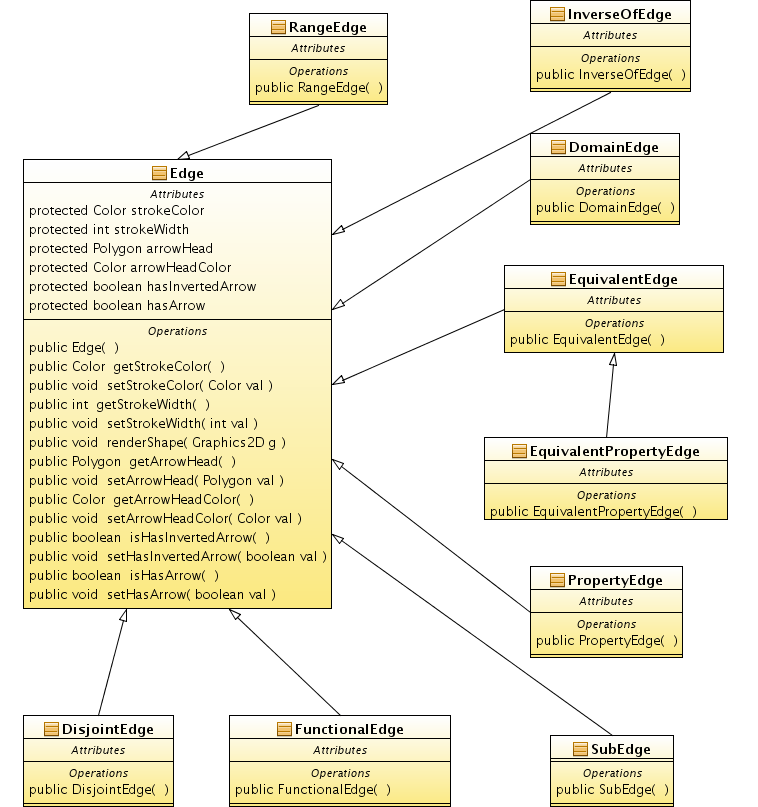
\includegraphics[width=\linewidth]{./modelowanie/OV_UML/EdgeClassDiagram.png}

\subsubsection{Opis klasy}

\begin{center}

\begin{longtable}{|m{3cm}|m{9cm}|} \hline

CE001 & Edge \\ \hline
Opis: &  Klasa reprezentująca prostą krawędź na grafie. Jest nadklasą dla pozostałych klas krawędzi.  \\ \hline
Klasy nadrzędne: &     \\ \hline
Atrybuty: & \begin{itemize}
\item Color strokeColor
\item  int strokeWidth 
\item boolean hasArrow
\item    boolean hasInvertedArrow
  \item  Polygon arrowHead
  \item Color arrowHeadColor
\end{itemize}
 \\ \hline
Metody: & \begin{itemize}
 \item    getStrokeColor () 
\item setStrokeColor (Color val)
  \item  getStrokeWidth () 
\item setStrokeWidth (int val) 
\item getArrowHead()
\item setArrowHead(Polygon arrowHead)
\item isHasArrow()
 \item setHasArrow(boolean hasArrow)
  \item isHasInvertedArrow()
\item setHasInvertedArrow(boolean hasInvertedArrow)
\item getArrowHeadColor()
 \item setArrowHeadColor(Color arrowHeadColor)
\end{itemize}
  \\ \hline
Realizowane wymagania: & WF006, WF007, WI004 \\ \hline
Priorytet: & bardzo ważne  \\ \hline

\multicolumn{2}{c}{} \\
 \hline

CE002 & DisjointEdge \\ \hline
Opis: & Klasa reprezentująca krawędź oznaczającą rozłączność klas (OWL Disjoint). \\ \hline
Klasy nadrzędne: & Edge    \\ \hline
Atrybuty: & %\begin{itemize}
 %\item 
%\end{itemize}
 \\ \hline
Metody: & %\begin{itemize}
 %\item 
%\end{itemize}
  \\ \hline
Realizowane wymagania: & WF006, WF007, WI004 \\ \hline
Priorytet: & ważne  \\ \hline

\multicolumn{2}{c}{} \\
 \hline

CE003 & DomainEdge  \\ \hline
Opis: & Klasa reprezentująca krawędź łączącą Property z klasą właściwości OWL DomainOf.   \\ \hline
Klasy nadrzędne: & Edge \\ \hline
Atrybuty: & %\begin{itemize}
 %\item 
%\end{itemize}
 \\ \hline
Metody: & %\begin{itemize}
 %\item 
%\end{itemize}
  \\ \hline
Realizowane wymagania: & WF006, WF007, WI004 \\ \hline
Priorytet: & ważne  \\ \hline

\multicolumn{2}{c}{} \\
 \hline

CE004 & EquivalentEdge \\ \hline
Opis: & Klasa reprezentująca krawędź oznaczającą równoznaczność (OWL Equivalent).    \\ \hline
Klasy nadrzędne: & Edge    \\ \hline
Atrybuty: & %\begin{itemize}
 %\item 
%\end{itemize}
 \\ \hline
Metody: & %\begin{itemize}
 %\item 
%\end{itemize}
  \\ \hline
Realizowane wymagania: & WF006, WF007, WI004 \\ \hline
Priorytet: & ważne  \\ \hline

\multicolumn{2}{c}{} \\
 \hline

CE005 & EquivalentPropertyEdge \\ \hline
Opis: & Klasa reprezentująca krawędź oznaczającą równoznaczność OWL Property (OWL EquivalentProperty).    \\ \hline
Klasy nadrzędne: & EquivalentEdge    \\ \hline
Atrybuty: & %\begin{itemize}
 %\item 
%\end{itemize}
 \\ \hline
Metody: & %\begin{itemize}
 %\item 
%\end{itemize}
  \\ \hline
Realizowane wymagania: & WF006, WF007, WI004 \\ \hline
Priorytet: & ważne  \\ \hline

\multicolumn{2}{c}{} \\
 \hline

CE006 & FunctionaltEdge \\ \hline
Opis: & Klasa reprezentująca krawędź łączącą wierzchołki InformationNode(CN012) z OWL Property, którego dotyczy.   \\ \hline
Klasy nadrzędne: & Edge    \\ \hline
Atrybuty: & %\begin{itemize}
 %\item 
%\end{itemize}
 \\ \hline
Metody: & %\begin{itemize}
 %\item 
%\end{itemize}
  \\ \hline
Realizowane wymagania: & WF006, WF007, WI004 \\ \hline
Priorytet: & ważne  \\ \hline

\multicolumn{2}{c}{} \\
 \hline

CE007 & InverseOfEdge \\ \hline
Opis: & Klasa reprezentująca krawędź oznaczającą odwrotność (OWL InverseOf).    \\ \hline
Klasy nadrzędne: & Edge    \\ \hline
Atrybuty: & %\begin{itemize}
 %\item 
%\end{itemize}
 \\ \hline
Metody: & %\begin{itemize}
 %\item 
%\end{itemize}
  \\ \hline
Realizowane wymagania: & WF006, WF007, WI004 \\ \hline
Priorytet: & ważne  \\ \hline

\multicolumn{2}{c}{} \\
 \hline

CE008 & PropertyEdge \\ \hline
Opis: &  Klasa reprezentująca krawędź oznaczającą relację między Property a klasą.   \\ \hline
Klasy nadrzędne: & Edge    \\ \hline
Atrybuty: & %\begin{itemize}
 %\item 
%\end{itemize}
 \\ \hline
Metody: & %\begin{itemize}
 %\item 
%\end{itemize}
  \\ \hline
Realizowane wymagania: & WF006, WF007, WI004 \\ \hline
Priorytet: & ważne  \\ \hline

\multicolumn{2}{c}{} \\
 \hline

CE009 & RangeEdge \\ \hline
Opis: & Klasa reprezentująca na grafie krawędź łączącą Property z klasą właściwości OWL Range.     \\ \hline
Klasy nadrzędne: & Edge    \\ \hline
Atrybuty: & %\begin{itemize}
 %\item 
%\end{itemize}
 \\ \hline
Metody: & %\begin{itemize}
 %\item 
%\end{itemize}
  \\ \hline
Realizowane wymagania: & WF006, WF007, WI004 \\ \hline
Priorytet: & ważne  \\ \hline

\multicolumn{2}{c}{} \\
 \hline

CE010 & SubEdge \\ \hline
Opis: & Klasa reprezentująca krawędź związku OWL SubClass pomiędzy klasami.   \\ \hline
Klasy nadrzędne: & Edge    \\ \hline
Atrybuty: & %\begin{itemize}
 %\item 
%\end{itemize}
 \\ \hline
Metody: & %\begin{itemize}
 %\item 
%\end{itemize}
  \\ \hline
Realizowane wymagania: & WF006, WF007, WI004 \\ \hline
Priorytet: & ważne  \\ \hline

%\multicolumn{2}{c}{} \\
% \hline


\end{longtable}

\end{center}

\subsection{Pakiet visualization }

\subsubsection{Diagram}

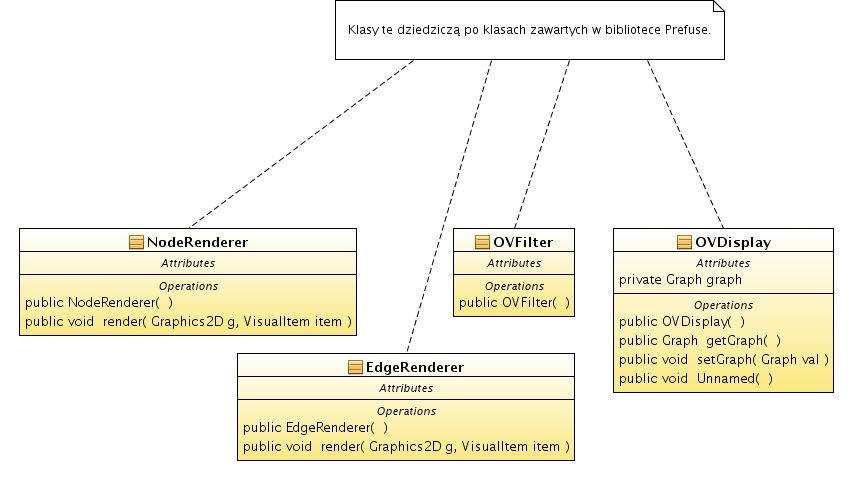
\includegraphics[width=\linewidth]{./modelowanie/OV_UML/VisualizationClassDiagram.png}

\subsubsection{Opis klasy}

\begin{center}
 

\begin{longtable}{|m{3cm}|m{9cm}|} \hline

CV001 & EdgeRenderer \\ \hline
Opis: & Klasa przeciążająca metody renderowania krawędzi grafu z biblioteki prefuse. \\ \hline
Klasy nadrzędne: &  prefuse.render.EdgeRenderer   \\ \hline
Atrybuty: & %\begin{itemize}
 %\item 
%\end{itemize}
 \\ \hline
Metody: & \begin{itemize}
 \item render(Graphics2D g, VisualItem item) - metoda renderująca krawędź
\end{itemize}
  \\ \hline
Realizowane wymagania: & WF001, WF008, WI004 \\ \hline
Priorytet: & ważne  \\ \hline

\multicolumn{2}{c}{} \\
 \hline

CV002 & NodeRenderer \\ \hline
Opis: & Klasa przeciążająca metody renderowania wierzchołków grafu z biblioteki prefuse.    \\ \hline
Klasy nadrzędne: &  prefuse.render.LabelRenderer   \\ \hline
Atrybuty: & %\begin{itemize}
 %\item 
%\end{itemize}
 \\ \hline
Metody: & \begin{itemize}
 \item render (Graphics2D g, VisualItem item) - metoda renderująca wierzchołek
\item drawString(Graphics2D g, FontMetrics fm, String text,
            boolean useInt, double x, double y, double w) - metoda wypisujaca na wierzchołku String
\end{itemize}
  \\ \hline
Realizowane wymagania: & WF001, WF008, WI004 \\ \hline
Priorytet: & ważne  \\ \hline

\multicolumn{2}{c}{} \\
 \hline

CV003 & OVDisplay \\ \hline
Opis: &  Klasa tworząca obiekt JComponent do umieszczenia na okienku JAVA zawierający wygenerowany graf z wizualizacją   \\ \hline
Klasy nadrzędne: &  prefuse.Display   \\ \hline
Atrybuty: & \begin{itemize}
 \item Graph graph - obiekt typu prefuse.data.graph zawierajacy dane o grafie do wyświetlenia. 
\end{itemize}
 \\ \hline
Metody: & \begin{itemize}
 \item getGraph() - zwarca graf z wyśiwetlanymi danymi
 \item setGraph(Graph graph) - nadpisuje obecny graf podanym
 \item generateGraphFromOWl(OWLOntology ont) - wpisuje do klasy obiekt Grpah wygenrowany na podstawie ontologii
	 
\end{itemize}
  \\ \hline
Realizowane wymagania: & WF001, WF002, WF008, WI004 \\ \hline
Priorytet: & ważne  \\ \hline

\multicolumn{2}{c}{} \\
 \hline

CV004 & OVFilter \\ \hline
Opis: & Klasa zawierająca filtry służace do wyświetlania danych w różnych zakresach    \\ \hline
Klasy nadrzędne: &     \\ \hline
Atrybuty: & %\begin{itemize}
 %\item 
%\end{itemize}
 \\ \hline
Metody: & %\begin{itemize}
 %\item 
%\end{itemize}
  \\ \hline
Realizowane wymagania: & WF001, WF008, WI004 \\ \hline
Priorytet: & ważne  \\ \hline

%\multicolumn{2}{c}{} \\
% \hline


\end{longtable}

\end{center}

\subsection{Pakiet graph}

\subsubsection{Diagram}

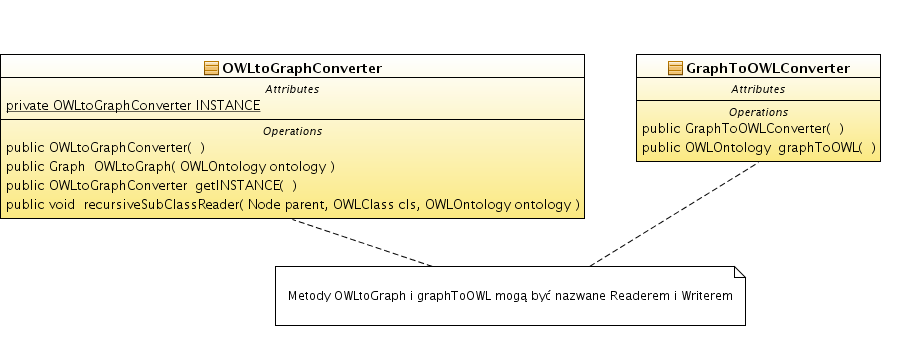
\includegraphics[width=\linewidth]{./modelowanie/OV_UML/GraphClassDiagram.png}

\subsubsection{Opis klasy}

\begin{center}
 


\begin{longtable}{|m{3cm}|m{9cm}|} \hline

CG001 & GraphToOWLConverter \\ \hline
Opis: & Klasa zawierająca metody pozwalające na przetwarzanie obiektów grafów z prefuse na obiekty OWL API. Klasa jest singletonem. \\ \hline
Klasy nadrzędne: &     \\ \hline
Atrybuty: & \begin{itemize}
 \item INSTANCE - instancja klasy GraphToOWLConverter 
\end{itemize}
 \\ \hline
Metody: & \begin{itemize}
	\item getInstance() - zwraca instancję klasy
	\item GraphToOWL(OWLOntology ontology) -Zamienia graf z biblioteki prefuse na ontologię zapisana w OWL API.
\end{itemize}
  \\ \hline
Realizowane wymagania: & WD001, WI004 \\ \hline
Priorytet: & ważne  \\ \hline

\multicolumn{2}{c}{} \\
 \hline

CG002 & OWLtoGraphConverter \\ \hline
Opis: & Klasa zawierająca metody pozwalające na przetwarzanie obiektów OWL API na obiekty prefuse. Klasa jest singletonem.\\ \hline
Klasy nadrzędne: &     \\ \hline
Atrybuty: & \begin{itemize}
 \item INSTANCE - instancja klasy GraphToOWLConverter 
\end{itemize}
 \\ \hline
Metody: & \begin{itemize}
	\item getInstance() - zwraca instancję klasy
	\item recursiveSubClassReader(Node parent, OWLClass cls,OWLOntology ontology ) - wczytuje do grafu OWL wszystkie klasy wraz z ich podklasami.
 	\item OWLToGraph(OWLOntology ontology) -Zamienia ontologię w OWL API na graf z biblioteki prefuse.
\end{itemize}
  \\ \hline
Realizowane wymagania: & WD001, WI004 \\ \hline
Priorytet: & ważne  \\ \hline

%\multicolumn{2}{c}{} \\
% \hline


\end{longtable}

\end{center}



\subsection{Pakiet utils}

\subsubsection{Diagram}

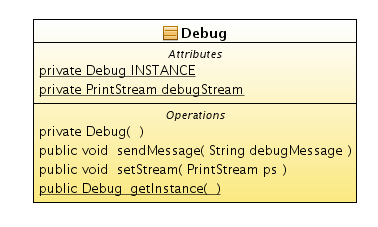
\includegraphics[width=0.5\linewidth]{./modelowanie/OV_UML/UtilsDiagram.png}

\subsubsection{Opis klasy}

\begin{center}

\begin{tabular}{|m{3cm}|m{9cm}|} \hline

CU001 & Debug \\ \hline
Opis: & Klasa do użycia przy debugowaniu, zapewnia strumien z błędami zwracanymi przez bibliotekę. Klasa jest singletonem.\\ \hline
Klasy nadrzędne: &     \\ \hline
Atrybuty: & \begin{itemize}
 \item INSTANCE - instacja klasy Debug
 \item Debug - Strumień do którego wpisywane są informacje potrzebne do debugowania
\end{itemize}
 \\ \hline
Metody: & \begin{itemize}
 \item getInstance() - zwraca instację klasy
 \item setStream(PrintStream ps) - ustawia podany strumień jako strumień na który zwracane będa błędy
 \item sendMessage(String s) - wysyła wiadomość na strumień do debugowania, jeżeli został wcześniej podpięty za pomocą funkcji setStream 	
\end{itemize}
  \\ \hline
Realizowane wymagania: & WF006, WF007, WI004 \\ \hline
Priorytet: & bardzo ważne  \\ \hline

%\multicolumn{2}{c}{} \\
% \hline
\end{tabular}
\end{center}

%\clearpage
%\phantomsubsection
%\addcontentsline{toc}{subsection}{Literatura}



\newpage


%opening
\section{Słownik}



\begin{center}
%budowanie tabeli
\begin{tabular}{|p{7cm}|p{7cm}|}
\hline
Symbol projektu: & Opiekun projektu:   \tabularnewline
3@KASK & mgr inż. Tomasz Boiński    \tabularnewline \hline
\multicolumn{2}{|l|}{Nazwa Projektu: } \tabularnewline
\multicolumn{2}{|l|}{Wizualizacja grafów za pomocą biblioteki Prefuse } \tabularnewline
\hline
\multicolumn{2}{l}{ } \tabularnewline %pusta linijka
\hline
Nazwa Dokumentu: & Nr wersji:   \tabularnewline
Słownik pojęć & 0.04 \tabularnewline \hline
Odpowiedzialny za dokument: & Data pierwszego sporządzenia:   \tabularnewline
Piotr Orłowski & 31.03.09 \tabularnewline \hline
Przeznaczenie: & Data ostatniej aktualizacji:   \tabularnewline
WEWNĘTRZNE & 15.05.09 \tabularnewline \hline
\end{tabular}
\end{center}

\begin{center}
\begin{tabular}{|c|p{4cm}|c|c|c|}
\multicolumn{5}{c}{\textbf{Historia dokumentu}} \tabularnewline \hline
\textbf{Wersja} & \textbf{Opis modyfikacji} & \textbf{Rozdział/strona} & \textbf{Autor modyfikacji} & \textbf{Data} \tabularnewline \hline
1 & Stworzenie zarysu słownika & wszystkie & Anna Jaworska & 31.03.09 \tabularnewline \hline
2 & Podstawowe pojęcia Semantic Web & Pojęcia ogólne & Piotr Orłowski & 31.03.09 \tabularnewline \hline
3 & Licencje wolnego oprogramwania & Pojęcia ogólne & Piotr Orłowski & 07.04.09 \tabularnewline \hline
4 & Uzupełnienie brakujących pojęć & wszystkie & Piotr Orłowski & 15.06.09 \tabularnewline \hline
& & & &\tabularnewline \hline
\end{tabular}
\end{center}



\subsection{Jak korzystać ze slownika}
Słownik został podzielony na dwie części:
\begin{itemize}
 \item pojęcia ogólne
 \item pojęcia specyficzne dla projektu.
\end{itemize}
Pojęcia zostały podane w sposób alfabetyczny. Słownik ten będzie rozwijany na bieżąco razem z rozwijaniem całego projektu.


\subsection{Pojęcia ogólne}
\begin{description}
	\item[agent] (lm. agenty) jednostka (np. program), działającą w pewnym środowisku, zdolna do komunikowania się, monitorowania swego otoczenia i podejmowania autonomicznych decyzji, aby osiągnąć cele określone podczas jej projektowania lub działania.
	\item[API] ang. Application Programming Interface, interfejs dla programów, zestaw poleceń, funkcji, metod, formatów i danych, które służą do wymiany informacji pomiędzy aplikacją i systemem operacyjnym oraz innymi programami lub sterownikami.
	\item[aplikacja standalone] to aplikacja, która do uruchomienia nie wymaga innych programów

	\item[BSD] Berkeley Software Distribution License, jedna z licencji zgodnych z zasadami Wolnego Oprogramowania stworzona na Uniwersytecie Kalifornijskim w Berkeley.
	\item[debugowanie] znany także jako odpluskwianie, proces szukania i naprawiania błędów	w programach komputerowych za pomocą specjalnych narzędzi do tego przeznaczonych.
	\item[GPL] GNU General Public License, jedna z licencji Wolnego Oprogramowania stworzona przez Richarda Stallmana i Ebena Moglena; zawiera zastrzeżenie, że wszystkie pochodne prace bazujące na kodzie wydanym na licencji GPL muszą być wydane na licencji GPL.

	\item[JAVA] Obiektowy język programowania; pojęcie używane czasem w sensie maszyny wirtualnej jezyka JAVA
	\item[javadoc] - generator dokumentacji stworzony przez firmę Sun Microsystems; narzędzie to generuje dokumentację kodu źródłowego Javy na podstawie zamieszczonych w kodzie komentarzy javadoc(do ich tworzenia używa się specjalnych tagów, które pozwalają na prawidłową interpretację informacji tam zawartej).
	\item[JVM] - Java Virtual Machine, maszyna wirtualna Javy, niezależny od platformy system uruchomieniowy dla programów napisanych w języku Java oraz innych (np. Jython) językach.

	\item[kapsułkowanie] - znane również jako hermetyzacja, enkapsulacja (z ang. encapsulation), jedno z założeń paradygmatu programowania obiektowego. Polega ono na ukrywaniu pewnych danych składowych lub metod obiektów danej klasy tak, aby były one dostępne tylko metodom wewnętrznym danej klasy oraz, ewentualnie, wybranym innym obiektom (np. klas zaprzyjaźnionych)..
	\item[KASK] Katedra Architektury Systemów Komputerowych WETI
	\item[krotka] - pojęcie matematyczne oznaczające uporządkowany, skończony zbiór elementów; w informatyce często używane do określenia rekordu bazy danych. W przypadku prefuse odnosi się do pojedynczego rekordu w tabeli.

	\item[metadane] są to dane opisujące inne dane, stosowane w celu ułatwienia korzystania z tych danych.
	\item[OCS] Ontology  Creation System - projekt realizowany w ramach grantu (tu id grantu) na KASK-u.
	\item[ontologia] dział filozofii starający się badać strukturę rzeczywistości i zajmujący się problematyką związaną z pojęciami bytu, istoty, istnienia i jego sposobów, przedmiotu i jego własności, przyczynowości, czasu, przestrzeni, konieczności i możliwości.

	\item[OWL] Web Ontology Language, jest to rozszerzenie RDFS. Język do opisu ontologii stworzony przez W3C.
	\item[pakiet] - tutaj jednostka organizacji klas w programowaniu obiektowym.
	\item[Prefuse] Biblioteka języka JAVA, pozwalająca na estetyczna prezentacje danych, w szczególności grafów

	\item[RDF] Resource Description Framework, jest specyfikacją W3C stosowaną do modelowania metadanych w postaci wyrażeń zawierających predykaty, klasy i podmioty; wyrażenia te tworzą graf skierowany.
	\item[RDFS] RDF Schema, język reprezentacji wiedzy oparty na RDF.
	\item[Sieć Semantyczna] ang. Semantic Web, projekt, który ma umożliwić łatwiejsze i bardziej logiczne wyszukiwanie przez maszyny i programy(agenty) danych w sieci Internet; znaczenie zasobów informacyjnych opisywane jest tu przy pomocy ontologii; do standardów rozwijanych wraz z Semantic Web należą m.in. OWL, RDF oraz RDFS

	\item[SHOIN/OWL] - język do wyrażania logiki opisowej ontologii.
	\item[strumień błędów] - specjalny strumień danych w programie, na który kierowane są informacje o błędach oraz ewentualnie przebiegu działania funkcji programu, w których istnieje ryzyko wystąpienia błędów.
	\item[SVN] SubVersioN - system kontroli wersji.

	\item[W3C] World Wide Web Consorcium - organizacja odpowiedzialna za ustalanie standardów dla metajęzyków.
 	\item[WETI/ETI] Wydział Elektroniki, Telekomunikacji i Informatyki Politechniki Gdańskiej
	\item[XML] ang. Extensible Markup Language, uniwersalny język formalny przeznaczony do reprezentowania różnych danych w ustrukturalizowany sposób.

\end{description}



\subsection{Pojęcia specificzne dla projektu}
\begin{description}
 	\item[kardynalność] tutaj występująca w języku OWL liczność elementu
	\item[klasa anonimowa] tutaj klasa będąca wynikiem operacji (np. logicznej) na innych klasach bądź powstała przez wyliczenie instancji.
 	\item[portalSubsystem] część projektu OCS, pozwala na wizualizację online plików OWL
\end{description}




\section{Załączniki}

\begin{enumerate}
 \item Notatka1
\item Notatka2
\item Notatka3
\item Notatka4
\item Notatka5
\item Notatka6
\item Notatka7
\item Notatka8
\item Notatka9
\item Notatka10
\item Notatka11
\item Notatka12
\item Notatka13
\item Notatka14
\item Notatka15
\item Notatka Specjalna
\item Plakat
\end{enumerate}







\end{document}
